% =========================================================================
% ColRadPy Theory Manual -- development branch working tree
% Build: python docs/source/theory/scripts/build_theory_manual.py
% Figures: python docs/source/theory/scripts/theory_examples.py
% =========================================================================
\documentclass[11pt,a4paper]{article}
\usepackage[utf8]{inputenc}
\usepackage[T1]{fontenc}
\usepackage{lmodern}
\usepackage{microtype}
\usepackage[a4paper,margin=2.5cm,headheight=14pt]{geometry}
\usepackage{amsmath,amssymb,mathtools}
\usepackage{graphicx}
\usepackage[section]{placeins}
\usepackage{booktabs,tabularx,longtable,array}
\usepackage{xcolor}
\usepackage{tikz}
\usetikzlibrary{arrows.meta,positioning,calc,fit,backgrounds}
\usepackage[font=small,labelfont=bf]{caption}
\usepackage{fancyhdr}
\usepackage[colorlinks=true,linkcolor=blue!50!black,citecolor=green!40!black,urlcolor=blue!50!black]{hyperref}
\newcommand{\vb}[1]{\boldsymbol{#1}}
\newcommand{\code}[1]{\texttt{\detokenize{#1}}}
\newcommand{\routine}[1]{\textsf{\detokenize{#1}}}
\newcommand{\dd}{\mathrm{d}}
\newcommand{\ee}{\mathrm{e}}
\newcommand{\nelec}{n_{\mathrm e}}
\newcommand{\nh}{n_{\mathrm h}}
\newcommand{\Te}{T_{\mathrm e}}
\newcommand{\units}[1]{\,\mathrm{#1}}
\newcommand{\revision}{\texttt{development}}
\definecolor{notebg}{RGB}{243,247,252}
\definecolor{noteframe}{RGB}{42,111,176}
\definecolor{warnbg}{RGB}{253,245,236}
\definecolor{warnframe}{RGB}{217,130,43}
\definecolor{aqua}{HTML}{2F9E8F}
\newsavebox{\notebox}
\newenvironment{implnote}[1][Implementation]{%
  \par\smallskip\noindent\begin{lrbox}{\notebox}\setlength{\fboxsep}{6pt}\begin{minipage}{\dimexpr\linewidth-2\fboxsep-2\fboxrule\relax}\small\textbf{#1.}\ }{%
  \end{minipage}\end{lrbox}\setlength{\fboxsep}{6pt}\fcolorbox{noteframe}{notebg}{\usebox{\notebox}}\par\smallskip}
\newenvironment{caveat}[1][Caveat]{%
  \par\smallskip\noindent\begin{lrbox}{\notebox}\setlength{\fboxsep}{6pt}\begin{minipage}{\dimexpr\linewidth-2\fboxsep-2\fboxrule\relax}\small\textbf{#1.}\ }{%
  \end{minipage}\end{lrbox}\setlength{\fboxsep}{6pt}\fcolorbox{warnframe}{warnbg}{\usebox{\notebox}}\par\smallskip}
\numberwithin{equation}{section}
\setlength{\parindent}{0pt}
\setlength{\parskip}{0.55em}
\renewcommand{\arraystretch}{1.15}
\setlength{\emergencystretch}{1.5em}
\pagestyle{fancy}
\fancyhf{}
\fancyhead[L]{\small ColRadPy Theory Manual}
\fancyhead[R]{\small\nouppercase{\leftmark}}
\fancyfoot[C]{\small\thepage}
\renewcommand{\headrulewidth}{0.4pt}
\hypersetup{pdftitle={ColRadPy Theory Manual},pdfsubject={Collisional radiative kinetics in the development branch}}

\begin{document}
\hypersetup{pageanchor=false}
\begin{titlepage}
\centering
\vspace*{3cm}
{\Huge\bfseries ColRadPy\par}
\vspace{0.6cm}
{\LARGE Theory Manual\par}
\vspace{0.4cm}
{\large Collisional radiative kinetics and spectral emission\par}
\vspace{2cm}
\begin{tabular}{rl}
Code version & 1.1 (\code{pyproject.toml})\\
Source branch & \revision\\
Source record & HEAD and file hashes in \code{provenance.json}\\
Code authors & C. A. Johnson and contributors (original code)\\
 & G. Ronchi (\revision{} branch)\\
Reference & C. A. Johnson, S. D. Loch and D. A. Ennis (2019)\\
Manual date & October 2026
\end{tabular}
\vfill
\begin{minipage}{0.82\textwidth}\small
This manual develops the rate equations, the elimination of excited states,
generalized collisional radiative coefficients, line emission, time-dependent
and charge-state solutions, and the energy-balance extension. Equations are mapped
to the routines that implement them. Blue notes explain implementation choices;
orange notes identify current limitations or qualifications. The worked checks
execute the development working tree; file hashes and the recorded HEAD are
given in \code{docs/source/theory/figures/provenance.json}.
\end{minipage}
\vspace{1.5cm}
\end{titlepage}
\pagenumbering{roman}
\hypersetup{pageanchor=true}
\begingroup\footnotesize\setlength{\parskip}{0pt}\tableofcontents\endgroup
\clearpage\pagenumbering{arabic}

\section{Physical framework and conventions}\label{sec:intro}

ColRadPy describes the populations and emission of atomic ions using a
generalized collisional-radiative (GCR) model~\cite{johnson,summers2006}.
Level-resolved atomic data determine the rates of excitation, decay,
ionization and capture. The resulting kinetic equations yield both the
populations of individual levels and effective coefficients for the
evolution of charge states. An ADAS ADF04 file provides the usual atomic
input, including level energies, radiative probabilities, effective
collision strengths and any available parent-resolved ionization,
recombination or charge-exchange data.

The basic model assumes a prescribed Maxwellian electron bath and
optically thin emission. Temperature and density are external parameters,
and emitted photons escape without further interaction. Ground and
metastable populations may remain independent dynamical variables, while
shorter-lived excited populations can be represented by their response
to these variables. This local kinetic description supplies coefficients
to transport and plasma models; radiative transfer, spatial transport and
the electron distribution function are outside its scope.

The competition between radiative and collisional rates connects the
coronal and high-density limits. At low density, spontaneous decay
dominates the removal of ordinary excited populations. As density
increases, reversible collisions can establish Boltzmann ratios within
a charge stage. Ionization and three-body recombination approach Saha
balance when the inverse rates and statistical weights are consistent.
These limiting behaviors provide physical checks on a calculation.
Implementation statements in this manual refer to the source recorded
with the accompanying figures and numerical checks~\cite{source}.

\subsection{Kinetic descriptions}

The level equations admit a full time-dependent solution and a
quasistatic reduction. The former follows every supplied population from
an initial state. The latter assumes that selected excited levels relax
rapidly and expresses their populations in terms of retained ground,
metastable and parent populations. Eliminating the excited levels also
produces effective rates, which couple adjacent ions in a charge-state
evolution model. The interpretation of each result follows from its
driving populations and normalization.

The development below proceeds from atomic rates to level kinetics,
quasistatic reduction, effective charge-state coefficients and emission.
The two-level example introduces the role of density and population
normalization before the general reduction. High-shell projection,
atomic-data preparation and kinetic-energy evolution extend this
framework in Sections~\ref{sec:projection}--\ref{sec:energy}.
The final section addresses applicability and verification; the
appendices document numerical algorithms, data conventions, the ADAS
production chain and the source and evidence supporting the manual.

\subsection{Calculation flow}

\begin{figure}[htbp]
\centering
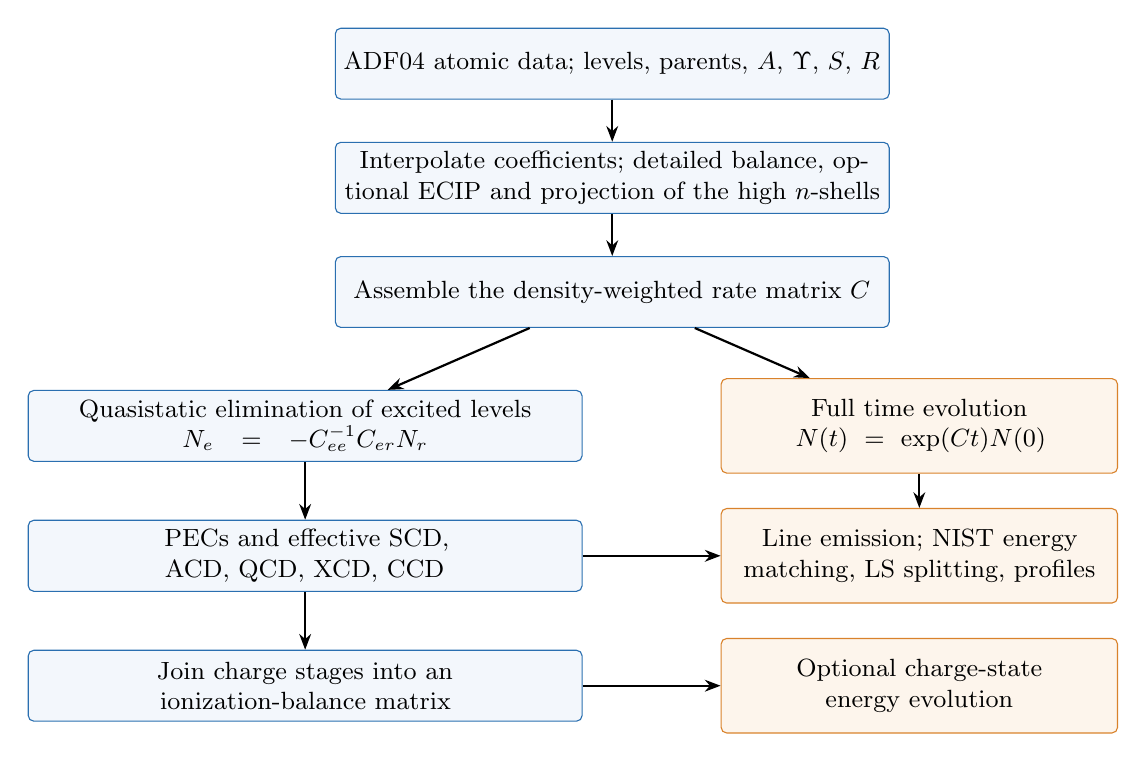
\begin{tikzpicture}[
 box/.style={draw=noteframe,rounded corners=2pt,fill=notebg,align=center,font=\small,minimum height=9mm,text width=68mm},
 side/.style={draw=warnframe,rounded corners=2pt,fill=warnbg,align=center,font=\small,minimum height=12mm,text width=48mm},
 arr/.style={-{Stealth[length=2mm]},thick}]
\node[box] (data) at (0,0) {ADF04 atomic data; levels, parents, $A$, $\Upsilon$, $S$, $R$};
\node[box] (rates) at (0,-1.45) {Interpolate coefficients; detailed balance, optional ECIP and projection of the high $n$-shells};
\node[box] (matrix) at (0,-2.9) {Assemble the density-weighted rate matrix $C$};
\node[box] (qs) at (-3.9,-4.6) {Quasistatic elimination of excited levels\\ $N_e=-C_{ee}^{-1}C_{er}N_r$};
\node[side] (td) at (3.9,-4.6) {Full time evolution\\ $N(t)=\exp(Ct)N(0)$};
\node[box] (gcr) at (-3.9,-6.25) {PECs and effective SCD, ACD, QCD, XCD, CCD};
\node[side] (spec) at (3.9,-6.25) {Line emission; NIST energy matching, LS splitting, profiles};
\node[box] (balance) at (-3.9,-7.9) {Join charge stages into an ionization-balance matrix};
\node[side] (energy) at (3.9,-7.9) {Optional charge-state energy evolution};
\draw[arr] (data)--(rates); \draw[arr] (rates)--(matrix);
\draw[arr] (matrix)--(qs); \draw[arr] (matrix)--(td);
\draw[arr] (qs)--(gcr); \draw[arr] (td)--(spec);
\draw[arr] (gcr)--(balance); \draw[arr] (gcr)--(spec);
\draw[arr] (balance)--(energy);
\end{tikzpicture}
\caption{The calculation paths are related but do not share the same population
normalization. The full matrix can also include parent or reservoir states;
their interpretation must be specified.}
\label{fig:flow}
\end{figure}

\subsection{Notation, indexing and units}\label{sec:units}

Let $N_i^{(z)}$ denote the number density of level $i$ in charge state
$z$. Bound levels are indexed by $i,j$, retained ground and metastable
levels by $\rho,\sigma$, and parents in charge state $z+1$ by $p,q$.
Matrix-block subscripts identify sets of states: $e$ denotes eliminated
excited levels, $m$ retained bound levels, and $r$ all retained states,
including the parents. Electron density is written explicitly as $\nelec$.

The defining matrix convention is
\begin{equation}\label{eq:matrix-convention}
 \frac{\dd N_i}{\dd t}=\sum_j C_{ij}N_j,
 \qquad C_{ij}:\ j\longrightarrow i.
\end{equation}
Each column therefore represents a source state and each row a
destination. Physical transfer rates give nonnegative off-diagonal
entries. Some stored coefficient arrays use a different index order,
documented in Appendix~\ref{sec:arrays}.

\begin{table}[htbp]\centering\small
\begin{tabularx}{\textwidth}{lXl}
\toprule Quantity & Meaning & Units\\\midrule
$\Te,T_i$ & Temperature represented as an energy & eV\\
$E_i,\ I_p$ & Tabulated level energies and parent thresholds & $\mathrm{cm}^{-1}$\\
$\nelec,\nh,N_i$ & Electron, neutral-donor and level densities & $\mathrm{cm}^{-3}$\\
$A_{u\ell}$ & Spontaneous emission probability & $\mathrm{s}^{-1}$\\
$q,S,\alpha^{\rm RR+DR},K$ & Two-body coefficients & $\mathrm{cm}^{3}\,\mathrm{s}^{-1}$\\
$\alpha^{(3)}$ & Three-body recombination coefficient & $\mathrm{cm}^{6}\,\mathrm{s}^{-1}$\\
$C$ & Density-weighted rate matrix & $\mathrm{s}^{-1}$\\
$\Upsilon$ & Effective collision strength & dimensionless\\
$\lambda$ & Internal wavelength & nm\\
PEC & Photon emission coefficient & $\mathrm{cm}^{3}\,\mathrm{s}^{-1}$\\
SCD, ACD, QCD, XCD, CCD & Effective two-body-form coefficients & $\mathrm{cm}^{3}\,\mathrm{s}^{-1}$\\
\bottomrule
\end{tabularx}
\caption{Core conventions. Effective coefficients may themselves depend on
density. The energy-transfer helper functions use SI densities and masses.}
\end{table}

The conversions needed repeatedly are
\begin{align}
 \Delta E_{\rm eV}&=\frac{100\,hc}{e}\,\Delta E_{\rm cm^{-1}}
   \simeq\frac{\Delta E_{\rm cm^{-1}}}{8065.544}, &
 T_{\rm K}&=\frac{e}{k_B}\,T_{\rm eV}\simeq11604.518\,T_{\rm eV},\label{eq:conversion}\\
 \lambda_{\rm vac,nm}&=\frac{10^7}{|E_u-E_\ell|_{\rm cm^{-1}}}, &
 n_{\rm m^{-3}}&=10^6n_{\rm cm^{-3}}.
\end{align}
The energy and temperature conversions use the CODATA values supplied by
\code{scipy.constants}; the factor 100 converts wavenumbers from
cm$^{-1}$ to m$^{-1}$. Several ADAS-derived rate expressions retain
their original rounded constants: 13.6058 eV and
$2.1716\times10^{-8}$ in Eq.~\eqref{eq:qdown}, 157890 K per rydberg in
ECIP, and $1.656742\times10^{-22}$ in Eq.~\eqref{eq:saha}. Numerical
reproduction should follow the constants used by the relevant routine.

Unless specified as tabulated wavenumbers, $\Delta E$, $\chi$ and FAC
energies in rate expressions are in eV. Consequently, ratios such as
$\Delta E/\Te$ are dimensionless. Expressions involving SI constants
require energies in joules, with $k_BT_{\rm K}=e\Te$. Photon energies
in power and electron-energy-loss coefficients are likewise in joules.
The wavelength conversion uses the tabulated wavenumber differences.

ADF04 level and parent identifiers are one-based, whereas Python indices
are zero-based. Thus \code{metas=[0,2]} retains the first and third bound
levels, leaving $[1,3,4,\ldots]$ as the eliminated set. This explicit
complement is needed when the retained levels are noncontiguous. Parent
identifiers must also be distinguished from their discovery order in
the input file.

\section{Atomic processes and rate coefficients}\label{sec:rates}

\subsection{Level structure and statistical weights}

Statistical weights reflect the resolution of the atomic model. An LS
term has weight $(2S+1)(2L+1)$, while a resolved-$J$ level has weight
$2J+1$. ColRadPy represents this through the ADF04 field
\code{atomic['w']} and uses $g_i=2w_i+1$ in rate construction. Parent
weights must follow the same resolution. Parent ionization thresholds
are specified in the file header, while level annotations identify
parentage channels; these two records need not enumerate the same
observed pathways~\cite{adf04}.

\begin{implnote}[Parent weights]
\routine{parent_statistical_weight} interprets LS and resolved-$J$
parent labels, including fractional $J$, to obtain $(2S+1)(2L+1)$ or
$2J+1$. Explicit ionization data may be present even when the associated
parentage annotations are incomplete, so channel identifiers and header
counts require consistent mapping.
\end{implnote}

\subsection{Maxwellian electron-impact excitation}

Electron-impact coefficients are averages of the cross-section over the
electron distribution. For a normalized energy probability density
$f_E$ in eV$^{-1}$, a cross-section $\sigma$ in cm$^2$ and electron
speed $v$ in cm/s, the excitation coefficient is
\begin{equation}
 q_{\ell u}=\int_{\Delta E}^{\infty}\sigma_{\ell u}(E)
       v(E)\,f_E(E)\,\dd E .
\end{equation}
Both the incident energy $E$ and threshold $\Delta E$ are in eV, giving
$q$ in cm$^3$/s. ADF04 expresses the nonrelativistic Maxwellian average
through the dimensionless effective collision strength
$\Upsilon_{\ell u}(T)$. For $u>\ell$, the downward coefficient and its
upward inverse are
\begin{align}
 q_{u\ell}(\Te)&=\frac{2.1716\times10^{-8}}{g_u}
        \sqrt{\frac{13.6058}{\Te}}\,\Upsilon_{\ell u}(\Te),\label{eq:qdown}\\
 q_{\ell u}(\Te)&=\frac{g_u}{g_\ell}
       \exp\!\left(-\frac{\Delta E}{\Te}\right)q_{u\ell}(\Te).
       \label{eq:qup}
\end{align}
The Boltzmann factor uses $\Delta E$ and $\Te$ in the same energy units.
The ratio of these coefficients gives
$N_u/N_\ell=(g_u/g_\ell)\exp(-\Delta E/\Te)$ when collisions control
the level ratio. This detailed-balance relation is the basis of the
within-stage Boltzmann limit. Section~\ref{sec:fac} describes the
corresponding treatment of cross-section data from FAC.

\begin{implnote}
\routine{make_electron_excitation_rates} interpolates $\Upsilon$ to the
requested temperatures. \routine{populate_cr_matrix} constructs the
upward and downward coefficients and applies the electron-density
factor. Boltzmann factors for excitation, ionization and three-body
recombination use the wavenumber-to-eV conversion in
Eq.~\eqref{eq:conversion}; ECIP retains the constants of \routine{r8ecip}.
\end{implnote}

\subsection{Spontaneous decay, ionization and recombination}

Spontaneous decay transfers population from $u$ to $\ell$ at rate
$A_{u\ell}N_u$, independently of electron density. Summation over the
accessible lower levels gives the total radiative loss rate,
$\Gamma_u=\sum_{\ell<u}A_{u\ell}$.

Ionization connects a bound level $i$ to a parent $p$ of the next charge
stage. In the supported ADF04 convention, the tabulated reduced
coefficient $\widetilde S_{ip}$ is related to the physical coefficient by
\begin{equation}\label{eq:reduced-ion}
 S_{ip}(\Te)=\widetilde S_{ip}(\Te)
            \exp[-\chi_{ip}/\Te],\qquad
 \chi_{ip}=\frac{100\,hc}{e}\,(I_p-E_i)\quad\text{(eV)}.
\end{equation}
The threshold factor is applied after interpolation of
$\widetilde S_{ip}$. The option \code{scale_file_ioniz} additionally
applies the input parentage factor to the interpolated reduced
coefficients, independently of the interpolation method, and is passed
to each stage by the ionization-balance calculation. Suspected
low-temperature placeholders are filtered before interpolation because
they would otherwise propagate into the inverse three-body rates.
Section~\ref{sec:interpolation} specifies these heuristic filters and
the warnings that identify affected channels and temperatures.

The file's radiative and dielectronic capture contributions are denoted
by $\alpha_{ip}^{\rm RR+DR}$. Including three-body recombination gives
the density-dependent coefficient
\begin{equation}\label{eq:recomb}
 R_{ip}(\Te,\nelec)=\alpha_{ip}^{\rm RR+DR}(\Te)
                       +\nelec\alpha_{ip}^{(3)}(\Te).
\end{equation}
The population-transfer rate is $\nelec R_{ip}N_p$. Radiative and
dielectronic capture therefore enter linearly in electron density,
whereas three-body capture enters quadratically. A zero or missing file
entry alone does not establish that the corresponding physical process
is absent.

Missing ionization channels may be supplemented with the approximate
ECIP model. For each parent $p$, \routine{ecip_rates} selects levels
annotated $\{p\}$ below that parent's threshold and passes temperatures
in kelvin to \routine{r8ecip}. Levels above the first ionization
threshold may thus contribute to higher-parent channels.
\routine{suppliment_with_ecip} uses parent annotations and zero entries
in the assembled ionization array to select the supplemented channels.
The resulting rates provide an approximate completion whose effect
should be included in atomic-model convergence studies.

\subsection{Three-body recombination and Saha detailed balance}\label{sec:saha}

Three-body recombination is related to ionization by equilibrium of
$i+e\rightleftharpoons p+e+e$. Equality of the forward and inverse
population-transfer rates requires
\begin{equation}
 N_i^*\nelec S_{ip}=N_p^*\nelec^2\alpha_{ip}^{(3)}.
\end{equation}
For nondegenerate, nonrelativistic electrons, the translational
partition factor then gives
\begin{align}
 \frac{\alpha_{ip}^{(3)}}{S_{ip}}
 &=\frac{g_i}{g_p}\frac{h^3}{2(2\pi m_e k_BT_{\rm K})^{3/2}}
                   \exp\!\left(\frac{\chi_{ip}}{\Te}\right)\nonumber\\
 &\simeq \frac{g_i}{g_p}\frac{1.6564\times10^{-22}}{\Te^{3/2}}
                   \exp\!\left(\frac{\chi_{ip}}{\Te}\right)
                   \units{cm^3}.\label{eq:saha}
\end{align}
The numerical form uses $\Te$ in eV, gives a volume in cm$^3$, and
includes the free-electron spin factor of two. The implementation uses
the nearby value $1.656742\times10^{-22}$. Evaluation of the first
form with SI constants instead gives m$^3$, requiring a factor $10^6$
for comparison. Its nonrelativistic basis is relevant when FAC forward
rates use relativistic thermal averages (Section~\ref{sec:fac}).

\begin{implnote}[Stable low-temperature evaluation]
The inverse rate is evaluated directly from reduced ionization data,
avoiding multiplication of an underflowed ionization coefficient by an
overflowing inverse exponential. For finite positive reduced data this
produces a finite positive value at fixed positive temperature; the
construction makes no assertion about a universal $T\to0$ limit.
\end{implnote}

\begin{implnote}[Standalone LTE helpers]
\routine{boltzmann_population} returns ground-relative level populations or
total-normalized fractions. \routine{saha_population} includes both stage
partition functions, ionization energy, electron mass, and electron density;
it returns $N_{z+1}/N_z$ or the two-stage ionized fraction. Energies are in
cm$^{-1}$, temperature in eV, and electron density in cm$^{-3}$.
\end{implnote}

\subsection{Thermal charge exchange}

Thermal charge exchange introduces a second bath: a donor species at
temperature $T_h$ and density $\nh$. Capture from parent $p$ into level
$i$ contributes $\nh K_{ip}(T_h)N_p^{\rm CX}$ to the bound-level balance.
The rate is controlled by donor density. \routine{make_cx_rates_from_file}
interpolates the donor-temperature data; its grid must be compatible
with the chosen electron-temperature/density grid or paired layout.

\section{Level-population equations and their solutions}\label{sec:matrix}

The level populations evolve under a rate matrix assembled from the
atomic coefficients and the appropriate bath densities. In the
source-column convention of Eq.~\eqref{eq:matrix-convention}, a transfer
contributes a positive destination-row entry and an equal loss on the
source diagonal. This construction connects the individual processes
to particle conservation and to the stationary and transient solutions.

For bound levels $i\ne j$, define $q_{j\to i}$ as the corresponding
electron-impact coefficient. Then
\begin{align}
 C_{ij}&=A_{j\to i}+\nelec q_{j\to i},\label{eq:bound-offdiag}\\
 C_{ii}&=-\sum_{j\ne i}(A_{i\to j}+\nelec q_{i\to j})
                  -\nelec\sum_pS_{ip}.\label{eq:bound-diag}
\end{align}
Radiative entries vanish for upward or forbidden transitions. Ionization
and recombination couple the bound levels to adjacent-charge parents
through
\begin{equation}
 C_{p i}=\nelec S_{ip},\qquad C_{i p}=\nelec R_{ip}.
\end{equation}
The parent diagonal contains the corresponding recombination loss into
the lower stage. When all destinations belong to the modeled system,
the gain and loss terms cancel in each source column:
\begin{equation}\label{eq:conservation}
 \sum_i C_{ij}=0\quad\hbox{for every source column }j,
 \qquad \frac{\dd}{\dd t}\sum_i N_i=0.
\end{equation}
An open subsystem may have nonzero column sums, provided its external
sources and sinks account for the population that crosses the boundary.

\begin{implnote}
\routine{populate_cr_matrix} stores the main generator in
\code{cr_matrix['cr']}; \code{A_ji} is stored with upper-level index first,
so radiative entries are transposed when inserted into the generator.
\code{cr_red} later contains only the selected excited-state block.
The separate \code{cr_loss} array holds only the level-loss diagonal of
that generator.
\end{implnote}

The quasistatic CX columns represent forcing by prescribed parent
populations and therefore contain gains without matching losses.
For full evolution, \routine{solve_time_dependent} assigns those gains
to the recombining-parent columns and includes the parent depletion on
the diagonal. The resulting generator obeys Eq.~\eqref{eq:conservation}.
The additional CX bookkeeping columns are then empty and require zero
initial populations and zero sources.

Nonnegative off-diagonal entries, the expected column sums and the
correct density powers are necessary checks on the kinetic model.
They test the physical assembly independently of the ability of a
linear solver to return a numerical solution.

\subsection{Time-dependent evolution and matrix exponentials}\label{sec:time}

For fixed plasma conditions and an optional constant source $s$,
\begin{equation}\label{eq:ode}
 \dot N=CN+s,\qquad
 N(t)=\ee^{Ct}N(0)+\int_0^t\ee^{C(t-u)}s\,\dd u.
\end{equation}
The exponential propagates the initial populations, while the integral
accumulates injection from the source throughout the interval. For
absolute populations, $s$ has units of density per unit time. This
solution is exact for fixed $C$ and constant $s$; numerical evaluation
is discussed in Appendix~\ref{app:numerical-methods}.

All requested times refer to the initial state at $t=0$. The choice of
that state encodes the physical preparation of the species. In the
surface-release example~\cite{johnson}, an initially ground-state
population develops metastable populations and time-dependent emission.
Relating this evolution to distance from the surface additionally
requires particle velocities and a transport geometry.

\subsection{Stationary solutions}

A normalized stationary population of a closed model satisfies
\begin{equation}
 C\pi=0,\qquad \vb1^{\mathsf T}\pi=1,\qquad \pi_i\ge0.
\end{equation}
For a unique stationary state, normalization replaces one redundant
balance equation. Rescaling the balance equations can help preserve
constraints associated with weak rates. If several disconnected closed
classes are present, normalization alone leaves their relative weights
undetermined; those weights depend on the initial condition.

Multiplication of $\pi$ by the conserved population recovers absolute
densities in a source-free closed system. With a prescribed source,
stationarity instead requires $CN+s=0$ and compatible population losses
or boundary conditions. A stationary collisional-radiative state may
remain far from LTE because it balances radiative escape as well as
collisions. The numerical stationary algorithms are described in
Appendix~\ref{app:numerical-methods}.

\subsection{A two-level density scan}

For a two-level ion with upward and downward coefficients $q_{01},q_{10}$
and radiative rate $A$, the excited population obeys
\begin{equation}
 \dot N_1=\nelec q_{01}N_0-(A+\nelec q_{10})N_1,
 \qquad N_0+N_1=N_{\rm ion}.
\end{equation}
At stationarity, excitation is balanced by radiative and collisional
return, giving $N_1/N_0=\nelec q_{01}/(A+\nelec q_{10})$.
Normalization to the conserved ion population yields
\begin{equation}
 f_1=\frac{\nelec q_{01}}{A+\nelec(q_{01}+q_{10})},\qquad
 \mathrm{PEC}_{10}=\frac{Aq_{01}}{A+\nelec(q_{01}+q_{10})}.
\end{equation}
The photon emissivity is $AN_1=\nelec N_{\rm ion}\mathrm{PEC}_{10}$.
Thus the PEC in this example is defined per ion total; a coefficient
per ground population would instead be $Aq_{01}/(A+\nelec q_{10})$.
At low density, the total-normalized PEC approaches $q_{01}$ and the
excited fraction grows linearly with density. At high density,
$f_1\to q_{01}/(q_{01}+q_{10})$ and the PEC decreases as $1/\nelec$.
The photon rate per ion nevertheless approaches the finite value
$Af_1$. The decrease of a density-normalized coefficient therefore
does not imply a vanishing photon yield.

\begin{figure}[htbp]\centering
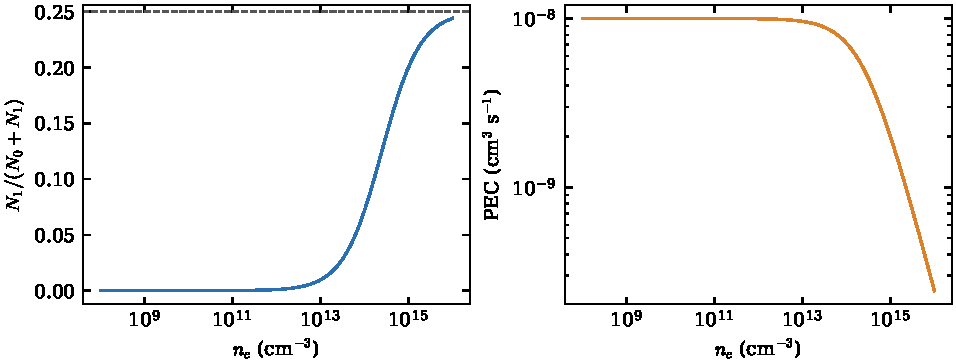
\includegraphics[width=\textwidth]{figures/two_level.pdf}
\caption{An analytic illustration with $A=10^7\,\mathrm{s}^{-1}$,
$q_{01}=10^{-8}$ and $q_{10}=3\times10^{-8}$ cm$^3$/s. The dashed line is
the high-density fraction $1/4$. These are illustrative coefficients, not
a fit to a specific atom or an execution of the ColRadPy atomic-data path.}
\end{figure}

\subsection{A conservative chain and a slow mode}

Consider three states connected by irreversible unit-rate transfers,
$0\to1\to2$. With time measured in seconds and rates in s$^{-1}$,
\begin{equation}\label{eq:chain}
 C=\begin{pmatrix}-1&0&0\\1&-1&0\\0&1&0\end{pmatrix},\quad
 N(0)=\begin{pmatrix}1\\0\\0\end{pmatrix},\quad
 N(t)=\begin{pmatrix}\ee^{-t}\\t\ee^{-t}\\1-(1+t)\ee^{-t}\end{pmatrix}.
\end{equation}
State 1 initially accumulates population and subsequently empties into
state 2, while the total population remains constant. Both the ColRadPy
solver and an independent SciPy exponential recover the analytic
solution. The $t e^{-t}$ contribution also tests the treatment of a
defective eigenbasis, discussed in Appendix~\ref{app:numerical-methods}.

\begin{figure}[htbp]\centering
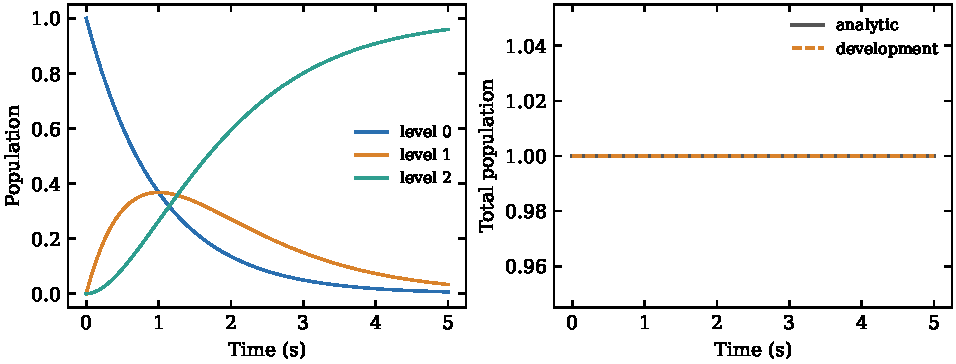
\includegraphics[width=\textwidth]{figures/chain.pdf}
\caption{Equal-rate chain: solid curves are analytic populations; dashed
curves are ColRadPy results. The right panel tests the conserved sum.
Agreement includes the $t\ee^{-t}$ contribution from the defective basis.}
\end{figure}

A complementary check concerns a very slow transition. For
$C=[[-r,0],[r,0]]$ with $r=10^{-12}$ s$^{-1}$ and $N(0)=(1,0)$,
the remaining initial-state population at $10^{12}$ s is $e^{-1}$.
The source solver with zero source reproduces this evolution and
agrees with the source-free calculation, confirming that the slow mode
is retained over the relevant observation time.

\section{Quasistatic reduction and population normalization}\label{sec:quasistatic}

The full kinetic system often contains excited levels that relax much
faster than the retained ground, metastable and parent populations.
Quasistatic elimination exploits this separation by replacing the fast
evolution equations with instantaneous balance. The excited populations
then follow the retained populations through a linear response, and
the remaining dynamics can be expressed with effective rates.

Partition the population vector into retained states $N_r$ and eliminated
excited states $N_e$. For a closed reduction, the retained set includes
both the selected bound levels and the adjacent-charge parents. In this
partition the full equations take the block form
\begin{equation}\label{eq:blocks}
 \frac{\dd}{\dd t}\begin{pmatrix}N_r\\N_e\end{pmatrix}
 =\begin{pmatrix}C_{rr}&C_{re}\\C_{er}&C_{ee}\end{pmatrix}
  \begin{pmatrix}N_r\\N_e\end{pmatrix}.
\end{equation}
When excited-state relaxation is fast compared with evolution of the drivers,
\begin{equation}\label{eq:qs}
 0=C_{ee}N_e+C_{er}N_r,
 \qquad N_e=-C_{ee}^{-1}C_{er}N_r.
\end{equation}
The matrix $-C_{ee}^{-1}C_{er}$ specifies the response to each retained
population. Its existence requires an invertible excited block, while
its physical use requires that the block relax on a sufficiently short
timescale. A slowly decaying eliminated mode can invalidate the
approximation even when the inverse is well defined. The relevant
time-scale and emission-convergence criteria are developed below.

Substitution into the retained equations gives the Schur complement
\begin{equation}\label{eq:schur}
 C_{\rm eff}=C_{rr}-C_{re}C_{ee}^{-1}C_{er}.
\end{equation}
The retained block contains the direct processes and losses, while the
second term accounts for excursions through the eliminated excited
manifold. Together they define the effective coefficients of
Section~\ref{sec:gcr}. Column-sum conservation is preserved for a closed
model, although the sum of the retained variables must still be
distinguished from a total that includes reconstructed excited
populations (Section~\ref{sec:ion-fractions}). The inverse notation is
convenient for the derivation; numerically the same response can be
obtained by solving $C_{ee}Y=-C_{er}$.

\subsection{Choosing retained levels and testing time-scale separation}\label{sec:metastables}

The GCR hierarchy distinguishes rapidly decaying autoionizing states,
ordinary excited levels and more slowly evolving ground and metastable
populations~\cite{summers2006}. At finite density, collisional
redistribution competes with radiative decay and autoionization, so
the relevant relaxation times belong to the coupled kinetic system.
The reduction is appropriate where these times are short compared with
the timescales on which the retained populations and plasma conditions
change. High-shell
projection applies the same reasoning to an auxiliary excited manifold
(Section~\ref{sec:projection}).

Spectroscopic metastability is consequently an initial guide to the
retained set, rather than a sufficient dynamical criterion~\cite{johnson}.
A weak radiative decay can permit substantial population accumulation,
while collisions and ionization shorten the effective relaxation time.
Conversely, strongly coupled ordinary excited levels may support a slow
collective mode. The retained manifold therefore depends on the plasma
conditions, initial state and observable under investigation.

For constant matrix blocks, write the instantaneous quasistatic response as
$N_e^{\rm qs}(t)=-C_{ee}^{-1}C_{er}N_r(t)$ and let
$\delta=N_e-N_e^{\rm qs}$. The exact lag equation is
\begin{align}
 \dot\delta&=C_{ee}\delta-\dot N_e^{\rm qs},\\
 \delta(t)&=\ee^{C_{ee}t}\delta(0)
       -\int_0^t\ee^{C_{ee}(t-u)}\dot N_e^{\rm qs}(u)\,\dd u.
       \label{eq:qs-lag}
\end{align}
The first term describes relaxation of the initial excited-state
departure from quasistatic balance; the integral describes the lag
induced by evolving drivers. After the initial transient has decayed,
accuracy depends on the ratio of excited relaxation time to driver
evolution time. Eigenvalues and eigenvectors of $C_{ee}$ characterize
this relaxation, subject to possible transient amplification in a
nonnormal system. A spectral gap alone is therefore insufficient as
an error bound. When plasma conditions vary, the response matrix also
changes and contributes to $\dot N_e^{\rm qs}$.

The adequacy of a retained manifold can be assessed by comparing full
and reduced solutions initialized with consistent retained populations,
then enlarging the manifold until the predicted emission converges over
the observation interval. Population magnitude alone is insufficient:
a weakly populated level may be an important feeder of a diagnostic
line. Relaxation modes are combinations of levels, so associating a
mode's decay rate with a single level requires inspection of its
eigenvector.

Published comparisons for Be I and Mo I illustrate this dependence on
species and conditions~\cite{johnson}. Table~\ref{tab:manifolds}
summarizes the effect of retaining metastables on the time-dependent
line emission relative to full level evolution.

\begin{table}[htbp]\centering\small
\begin{tabularx}{\textwidth}{l l X}
\toprule Published case & Plasma conditions & Reported observation\\\midrule
Be I & $\Te=20$ eV, $\nelec=10^{13}$ cm$^{-3}$ &
Retaining the important metastable substantially improves the time-dependent
line-emission prediction over a ground-only reduction.\\
Mo I & $\Te=8$ eV, $\nelec=5\times10^{11}$ cm$^{-3}$ &
Even a ten-metastable reduction does not reproduce the full
time-dependent line history.\\
\bottomrule
\end{tabularx}
\caption{Retained sets compared with the full time-dependent
model~\cite{johnson}, not rerun for this manual. They do not set a universal
number of retained levels for either species.}\label{tab:manifolds}
\end{table}

The clearer separation between slow and fast modes in Be permits an
effective reduction with a small retained manifold. The more gradual
relaxation spectrum in Mo makes that reduction less successful.
These examples motivate convergence tests for the chosen observable
and conditions, rather than a fixed number of retained levels for
either species. A ground-only reduction also removes the independent
evolution of metastable fractions.

\subsection{Separate excitation, recombination and CX drivers}\label{sec:cxdrivers}

The retained populations drive excited levels through distinct physical
channels. Separating bound-level forcing, electron recombination and
charge exchange gives
\begin{equation}
 0=C_{ee}N_e+C_{e m}N_m+\nelec R_{e p}N_p
                                +\nh K_{e p}N_p^{\rm CX}.
\end{equation}
The corresponding dimensionless responses are
\begin{align}
 F&=-C_{ee}^{-1}C_{em}, &
 G&=-C_{ee}^{-1}\nelec R_{ep}, &
 H&=-C_{ee}^{-1}\nh K_{ep},\label{eq:responses}\\
 N_e&=FN_m+GN_p+HN_p^{\rm CX}.\nonumber
\end{align}
Each column describes the population response of the eliminated manifold
to one prescribed driver. Multiplication by the actual driver populations
and summation recover the physical excited populations. A response
column has no probability normalization of its own.

\begin{implnote}
\routine{solve_quasi_static} stores the forcing as
\code{beta}$=-C_{er}$ and evaluates
\code{pops}$=C_{ee}^{-1}\code{beta}$. Columns are ordered as
excitation, recombination and CX when enabled.
\code{processed['F']} omits the additional inverse-density factor
of some ADAS conventions and follows the selected excitation
normalization. It equals the unnormalized $F$ in
Eq.~\eqref{eq:responses} when normalization is disabled; the mapping
to other stored conventions is given in Section~\ref{sec:normalization}.
\end{implnote}

\begin{implnote}[CX-only construction]
When CX is enabled but both radiative and three-body recombination are
disabled, the CX columns still follow the parent columns, which the
generator keeps whether or not recombination is used.
\end{implnote}

\subsection{Normalization is a choice of driving population}\label{sec:normalization}

Normalization specifies the population to which a response or emission
coefficient refers. Absolute level densities are recovered by weighting
the independent response columns in Eq.~\eqref{eq:responses}; level
fractions additionally require a defined population total. The
conventions most frequently used below are summarized in the table.

\begin{table}[htbp]\centering\small
\begin{tabularx}{\textwidth}{lXX}
\toprule Quantity & Denominator & Interpretation\\\midrule
$N_i$ & None & Absolute level density, cm$^{-3}$\\
$F_{i\rho}$ & Retained bound driver $N_\rho$ & Excited response of that driver's column\\
$G_{ip},\ H_{ip}$ & Parent driver $N_p$ or $N_p^{\rm CX}$ & Capture-driven response in another charge stage\\
$N_i/N_{\rm stage}$ & Total population in the stage & Level fraction after all contributions are assembled\\
\bottomrule
\end{tabularx}
\caption{Population conventions. Responses are dimensionless but their
column sums need not be one.}
\end{table}

For a single ground driver and no capture contribution,
$N_i=F_{i0}N_0$ and $N_{\rm ion}=N_0+\sum_iN_i$. Therefore
\begin{equation}
 \frac{N_0}{N_{\rm ion}}=\frac{1}{1+\sum_iF_i},\qquad
 \frac{N_i}{N_{\rm ion}}=\frac{F_i}{1+\sum_jF_j}.
\end{equation}
Here $F_i=F_{i0}$. The rescaling converts an excitation response per
ground population into a level fraction per ion total. Recombination
responses retain a parent population from the next charge stage as
their denominator. For example, parent-driven injection
$\nelec\alpha=2$ s$^{-1}$ into a level with loss rate $A=1$ s$^{-1}$
gives $N_i/N_p=2$. Such a value is consistent with a linear response
and illustrates the importance of preserving the separate GCR
drivers~\cite{adasreport}.

For an excitation driver $\rho$, define
\begin{equation}\label{eq:stored-normalization}
 d_\rho=\begin{cases}
 (1+\sum_{i\in e}F_{i\rho})^{-1},&\text{excitation normalization on},\\
 1,&\text{excitation normalization off}.
 \end{cases}
\end{equation}
In this definition $F$ is the unnormalized response of
Eq.~\eqref{eq:responses}. The normalization applied to stored
excitation quantities is consequently
\begin{align}
 F^{\rm stored}_{i\rho}&=d_\rho F_{i\rho}, &
 \mathrm{PEC}^{\rm stored,exc}_{u\ell,\rho}
   &=d_\rho\mathrm{PEC}^{\rm exc}_{u\ell,\rho},\nonumber\\
 \mathcal S^{\rm stored}_{\rho p}
   &=d_\rho S_{\rho p}+\sum_iS_{ip}F^{\rm stored}_{i\rho}
    =d_\rho\mathcal S_{\rho p}.\label{eq:stored-scd}
\end{align}
Both the direct and excited-mediated ionization terms carry the same
factor $d_\rho$. Using a normalized \code{processed['F']} with an
unscaled direct term would therefore mix population conventions.
The original response columns are available in
\code{processed['pops_no_norm']}, with excitation columns first.
Recombination and CX responses $G,H$ are unaffected by this excitation
normalization.

For a single ground driver without capture, $d_0=N_0/N_{\rm ion}$,
and the normalized excitation coefficient multiplies $N_{\rm ion}$.
With several retained levels, separate normalization of each column
describes its driver and associated excited response in isolation.
A physical mixture is instead assembled from unnormalized responses
and the actual retained populations.

\begin{implnote}[Selecting the stored convention]
Excitation normalization defaults on for one retained metastable and
off for several; parent-driven recombination and CX columns keep
their independent denominators. \code{default_pop_norm=False}
reverses this selection. The actual convention is recorded in
\code{processed['driving_populations_norm']}. Effective-coefficient
derivations use unnormalized responses, with the stored SCD mapping
specified by Eq.~\eqref{eq:stored-scd}.
\end{implnote}

\subsection{Retained fractions and total ion fractions}\label{sec:ion-fractions}

Normalization of retained populations across all modeled charge stages
gives $f_a^{(r)}=N_a/\sum_{b\in r}N_b$. Converting these retained
fractions to fractions of the full modeled population requires the
excited-state contribution. For one charge stage the reconstructed
bound-level total is
\begin{equation}\label{eq:stage-total}
 N_{\rm stage}=\sum_\rho N_\rho+
  \sum_{i\in e}\left(\sum_\rho F_{i\rho}N_\rho+
                 \sum_p G_{ip}N_p+\sum_p H_{ip}N_p^{\rm CX}\right).
\end{equation}
All terms in this reconstruction use unnormalized responses and a
common absolute scale for the driving populations. The sum includes
the explicit bound levels; populations in the projected high shells
remain eliminated and are not counted separately.

When the omitted excited population is small, retained and total
fractions are close. Otherwise, total ion fractions and power per ion
of the element require reconstruction of each stage and normalization
by the sum of those stage totals. Excitation-normalized single-ground
coefficients account for the excited population associated with that
driver, while capture-driven excited populations remain parent-driven
responses (Section~\ref{sec:stage}). Equation~\eqref{eq:stage-total}
makes both contributions explicit.

This distinction also affects transients. The Schur complement
conserves the retained sum, whereas the reconstructed total may vary
because the eliminated population derivatives were neglected in the
reduced equations. Appreciable transient storage in excited levels
therefore calls for a larger retained manifold or full level evolution;
renormalization alone does not supply the missing dynamics.

\section{Effective coefficients and charge-state evolution}\label{sec:gcr}

The Schur complement converts the response of the eliminated levels
into effective transfers between retained states. Its bound-to-parent,
parent-to-bound and within-manifold blocks define the GCR coefficients
summarized below. Division by the appropriate bath density expresses
these rates in cm$^3$/s. Throughout the derivation, the responses of
Eq.~\eqref{eq:responses} are unnormalized and the retained populations
are prescribed explicitly. Stored array orientations are documented
in Appendix~\ref{sec:arrays}.

\begin{table}[htbp]\centering\small
\begin{tabularx}{\textwidth}{lllX}
\toprule Coefficient & Source & Destination & Included pathways\\\midrule
SCD & Bound $\rho$ & Parent $p$ & Direct ionization and ionization after bound excitation\\
ACD & Parent $p$ & Bound $\rho$ & Electron capture and stabilization through excited levels\\
CCD & CX parent $p$ & Bound $\rho$ & Donor-driven capture and subsequent stabilization\\
QCD & Bound $\sigma$ & Bound $\rho$ & Direct mixing and redistribution through excited levels\\
XCD & Parent $p$ & Parent $q$ & Capture and re-ionization through the lower ion\\
\bottomrule
\end{tabularx}
\caption{Physical meaning of the effective transfers. SCD, ACD, QCD and
XCD multiply $\nelec$; CCD multiplies $\nh$. Projection can add the
high-shell pathways described in Section~\ref{sec:projection}.}
\end{table}

\subsection{SCD: effective ionization}

For a retained bound level $\rho$ and destination parent $p$,
\begin{equation}
 \mathcal S_{\rho p}=S_{\rho p}+\sum_iS_{ip}F_{i\rho}.
\end{equation}
The first term is direct ionization of the retained level; the second
accounts for population transferred through excited levels before
ionization. The effective contribution to $C_{\rm eff}$ from $\rho$
to $p$ is $\nelec\mathcal S_{\rho p}$.

\subsection{ACD and CCD: effective capture}

The capture coefficient from parent $p$ into retained level $\rho$ is
\begin{equation}
 \mathcal A_{\rho p}=R_{\rho p}
              -\sum_{ij}C_{\rho i}(C_{ee}^{-1})_{ij}R_{jp}.
\end{equation}
The indirect term describes capture into the excited manifold followed
by redistribution and radiative stabilization into $\rho$. Replacing
$R$ by $K$ gives the charge-exchange coefficient $\mathcal C_{\rho p}$
(CCD). ACD multiplies electron density and CCD multiplies donor density;
an ionization matrix expressed per electron density therefore contains
$(\nh/\nelec)\mathcal C$ for charge exchange.

\subsection{QCD: redistribution within a retained bound manifold}

For two different retained bound levels,
\begin{equation}
 \mathcal Q_{\sigma\to\rho}
 =\frac{C_{\rho\sigma}+\sum_iC_{\rho i}F_{i\sigma}}{\nelec},
 \qquad \rho\ne\sigma.
\end{equation}
QCD includes both direct retained-level mixing and redistribution
through the excited manifold. Its stored diagonal is zero; the
corresponding source losses are included when the charge-state
generator is assembled.

\subsection{XCD: redistribution between parent metastables}\label{sec:xcd}

A parent $p$ can recombine into an excited level of the lower stage and then
ionize into a different parent $q$. The coefficient for this path is
\begin{equation}\label{eq:xcd}
 \mathcal X_{p\to q}=-\sum_{ij}C_{qi}(C_{ee}^{-1})_{ij}R_{jp}
       =-\nelec\sum_{ij}S_{iq}(C_{ee}^{-1})_{ij}R_{jp},\qquad p\ne q.
\end{equation}
The factor $\nelec$ arises because ionization out of the excited
manifold is a density-weighted rate. The resulting units are
\begin{equation}
 [\nelec S][C_{ee}^{-1}][R]
  =(\mathrm{s}^{-1})(\mathrm s)(\mathrm{cm}^3\,\mathrm{s}^{-1})
  =\mathrm{cm}^3\,\mathrm{s}^{-1}.
\end{equation}
Equivalently, XCD is the off-diagonal parent block of the Schur
complement divided by electron density. Its contraction requires a
common eliminated-level ordering for the recombination rows and
$C_{ee}$. The density factor agrees with Eq.~17 of Summers et
al.~\cite{summers2006}. High-shell projection adds the parent transfer
$X^{\rm ind}_{qp}$ defined in Eq.~\eqref{eq:expansion}. This correction
is stored with destination first and is transposed on addition to the
source-first XCD array (Appendix~\ref{sec:arrays}).

\begin{implnote}[XCD contraction]
The contraction uses $\nelec S$ and selects recombination rows by the actual
eliminated-level map, including noncontiguous metastable selections such as
$[0,2]$. The resulting coefficient has units cm$^3$/s and agrees with the
parent block of the direct Schur complement divided by electron density.
\end{implnote}

\subsection{XCD checked by direct elimination}

The bundled Be II file is solved with metastables $[0,1]$, temperatures
$[5,20]$ eV and densities $[10^{12},10^{14}]$ cm$^{-3}$, with both
recombination mechanisms and ionization enabled. At the first grid point,
the off-diagonal parent block of Eq.~\eqref{eq:schur}, formed with a linear
solve rather than the stored inverse and divided by $\nelec$, agrees with the
stored XCD$[1,0]$ (Table~\ref{tab:checks}); both are in cm$^3$/s. A separate
test with the noncontiguous metastables $[0,2]$ covers the row selection.

\subsection{Ionization balance across charge stages}\label{sec:ionbalance}

Effective coefficients from successive ions form a coupled
charge-state model. Collecting their retained populations into $x$
gives, at fixed plasma conditions,
\begin{equation}
 \dot x=Mx+s,\qquad M=\nelec B.
\end{equation}
The coefficient matrix $B$ has units cm$^3$/s. SCD and ACD couple
adjacent stages, while QCD redistributes retained populations within
the ion from which it was calculated. XCD adds redistribution within
the parent stage through excursions into the lower ion. A given stage
can therefore receive its own QCD contribution and the XCD contribution
calculated from the preceding stage.

\subsubsection{Matrix assembly and density factors}

Each off-diagonal coefficient is accompanied by an equal source-diagonal
loss, giving $\vb1^{\mathsf T}B=0$ for a closed model. Charge-exchange
entries contain $(\nh/\nelec)\mathcal C$, so multiplication of $B$ by
$\nelec$ restores the donor-density rate $\nh\mathcal C$.

\begin{implnote}
\routine{populate_ion_matrix} stores $B$ in \code{ion_matrix}, despite that
name suggesting a density-weighted rate. \routine{solve_no_source} and
\routine{solve_source} multiply by the electron-density grid before invoking
the matrix-exponential solvers. Do not apply the density multiplier a second
time when interpreting their populations.
\end{implnote}

\subsubsection{Ionization age}

For constant electron density, the ionization age is $\tau=\nelec t$.
At fixed temperature, density-independent $B$ gives
$x(\tau)=\exp(B\tau)x(0)$. In a GCR model, collisional quenching and
three-body capture can introduce an explicit density dependence into
$B$. Equal ionization age then need not produce equal charge-state
fractions at different densities.

\begin{implnote}[Ionization-age grids]
The wrapper constructs times as $t=\tau/\nelec$ with axes
\emph{density, time} when there are multiple densities; one density uses a
one-dimensional time array. This agrees with the matrix-exponential solver's
grid convention, including singleton axes.
\end{implnote}

\subsection{Stage-to-stage coefficients}\label{sec:stage}

Charge-state kinetics can retain separate metastable populations or
reduce each stage to one population. Two reductions are ground
condensation and contraction with prescribed metastable fractions.
Each requires a prescription for the populations within the stage, and
their treatment of excitation-fed and capture-fed
populations determines the meaning of the resulting stage
coefficients~\cite{summers2006}.

\subsubsection{Resolved metastables and ground condensation}

In the resolved description, each selected ground or metastable level
has an independent population. QCD and XCD determine redistribution,
and SCD, ACD and CCD connect adjacent stages. The within-stage
fractions consequently follow from the coupled kinetics.

Ground condensation eliminates all bound levels except the ground of
each stage. Under the single-driver normalization of
Section~\ref{sec:normalization}, the stage variable includes the
excited population driven by ground excitation. Capture-driven excited
populations remain responses to the next stage, and ACD measures the
capture flow reaching the retained ground. This conventional CR
reduction therefore uses the stage-population convention described in
Section~\ref{sec:ion-fractions}.

\subsubsection{Contraction with metastable fractions}

A second construction contracts resolved coefficients with prescribed
metastable fractions. Writing the ground-relative ratios as
$\eta_\rho=N_\rho/N_g$ with $\eta_g=1$ gives
$f_\rho=\eta_\rho/\sum_\sigma\eta_\sigma$. If $f_p^+$ denotes the
corresponding fractions in the recombining stage, the contracted
coefficients are
\begin{equation}\label{eq:unresolved}
 \mathcal S_{\rm stage}=\sum_\rho f_\rho\sum_p\mathcal S_{\rho p},\qquad
 \mathrm{PLT}_{\rm stage}=\sum_\rho f_\rho\,\mathrm{PLT}_\rho,\qquad
 \mathcal A_{\rm stage}=\sum_p f_p^+\sum_\rho\mathcal A_{\rho p}.
\end{equation}
SCD and PLT are weighted by the fractions of the ionizing or emitting
stage. ACD is weighted by the recombining-parent fractions and summed
over bound destinations; CCD uses the same construction. The parent
fractions also weight PRB and PRC. The resulting model has one
population per stage, with no separate QCD or XCD entries, although
redistribution can influence the fractions used in the contraction.

The ADAS GCR-project contraction uses MET ratios obtained from a
within-stage model with a prescribed ground driver and no capture
feeding from the next stage (Appendix~\ref{sec:adf11adas}). For one
metastable $\mu$, its quasistatic balance gives
\begin{equation}\label{eq:met}
 \eta_\mu=\frac{\mathcal Q_{g\to\mu}}
             {\mathcal Q_{\mu\to g}+\sum_p\mathcal S_{\mu p}}.
\end{equation}
With several metastables, their responses to the ground driver are
obtained from a linear system. These excitation-only ratios describe
the specified within-stage balance and can differ from the fractions
established by capture and ionization in a coupled plasma.

\subsubsection{When capture feeding changes the fractions}

The effect of capture feeding can be seen directly in the same
ground--metastable system. Including capture from the next stage,
while neglecting CX and other feeding channels in this illustration,
gives the stationary metastable balance
\begin{equation}\label{eq:met-balance}
 0=\mathcal Q_{g\to\mu}N_g
   -\left(\mathcal Q_{\mu\to g}+\sum_p\mathcal S_{\mu p}\right)N_\mu
   +\sum_p\mathcal A_{\mu p}N_p^+,
\end{equation}
after dividing the rate equation by $\nelec$. It follows that
\begin{equation}\label{eq:met-plasma}
 \frac{N_\mu}{N_g}=\eta_\mu+
 \frac{\sum_p\mathcal A_{\mu p}N_p^+}
      {(\mathcal Q_{\mu\to g}+\sum_p\mathcal S_{\mu p})N_g}.
\end{equation}
The additional term is negligible when capture feeding is small
relative to $\mathcal Q_{g\to\mu}N_g$. The parent abundance alone is
therefore insufficient to assess the excitation-only approximation.
Substantial capture changes the metastable population available for
re-ionization, whereas ground condensation assigns that population
through a different retained variable. The accuracy of either
reduction depends on the ion and conditions. In the resolved system,
XCD from the preceding stage also contributes to redistribution of
these populations~\cite{summers2006}.

\begin{implnote}[Stage contraction]
For ADF04 inputs, \code{use_met=True} in \routine{ionization_balance}
contracts resolved coefficients using fractions from
\routine{metastable_fractions}, calculated from each stage's QCD and
SCD. The default \code{use_met=False} preserves the supplied retained
manifolds. Matching unresolved ADAS coefficients additionally requires
consistent MET data, interpolation and atomic inputs.
\end{implnote}

Retaining the metastables allows these fractions to evolve within the
coupled model. Its accuracy remains subject to the atomic data,
time-scale separation and population conventions specified above.

\section{Emission, power and spectroscopic diagnostics}\label{sec:emission}

Spectroscopic observables follow directly from the level populations.
A one-photon transition produces photons at rate $A_{u\ell}N_u$ per
unit volume, and each photon carries energy $\Delta E_{u\ell}$.
Substitution of the quasistatic responses separates the emissivity
into excitation, recombination and charge-exchange contributions.
Their coefficients inherit the driving-population convention of
Section~\ref{sec:normalization}.

To compare notation, the response functions used in Section~1.2.2 of
Summers et al.~\cite{summers2006} are
$\mathcal F^{\rm (exc)}_{u\rho}=F_{u\rho}/\nelec$ and
$\mathcal F^{\rm (rec)}_{up}=G_{up}/\nelec$. They include an additional
inverse electron-density factor relative to the dimensionless
responses defined here. Stored excitation quantities may also carry
the normalization of Eq.~\eqref{eq:stored-normalization}.

\subsection{Photon emissivity coefficients}

For optically thin emission, the angle-integrated photon emissivity
of a one-photon line $u\to\ell$ is $A_{u\ell}N_u$. Resolving the
upper-level population by driver gives
\begin{equation}\label{eq:emissivity}
 \epsilon_{u\ell}=A_{u\ell}N_u
 =\nelec\sum_\rho N_\rho\mathrm{PEC}^{\rm exc}_{u\ell,\rho}
  +\nelec\sum_pN_p\mathrm{PEC}^{\rm rec}_{u\ell,p}
  +\nh\sum_pN_p^{\rm CX}\mathrm{PEC}^{\rm CX}_{u\ell,p}
 \quad[\mathrm{photons}\,\mathrm{cm}^{-3}\,\mathrm{s}^{-1}].
\end{equation}
Factoring out the bath density and driving population defines the
photon emissivity coefficients, in cm$^3$/s:
\begin{align}
 \mathrm{PEC}^{\rm exc}_{u\ell,\rho}&=A_{u\ell}F_{u\rho}/\nelec,\label{eq:pec-exc}\\
 \mathrm{PEC}^{\rm rec}_{u\ell,p}&=A_{u\ell}G_{up}/\nelec,\label{eq:pec-rec}\\
 \mathrm{PEC}^{\rm CX}_{u\ell,p}&=A_{u\ell}H_{up}/\nh.\label{eq:pec-cx}
\end{align}
For a retained upper level $\sigma$, the population is already an
independent variable. Its response to a retained bound driver $\rho$
is $\delta_{\sigma\rho}$, so its radiative transitions have
\begin{equation}\label{eq:pec-meta}
 \mathrm{PEC}^{\rm exc}_{\sigma\ell,\rho}=\delta_{\sigma\rho}A_{\sigma\ell}/\nelec,
 \qquad
 \mathrm{PEC}^{\rm rec}_{\sigma\ell,p}=\mathrm{PEC}^{\rm CX}_{\sigma\ell,p}=0.
\end{equation}
The same emissivity can be expressed per ion total by changing the
coefficient's denominator. For a single ground driver without capture,
the corresponding excitation PEC is $d_0\mathrm{PEC}^{\rm exc}$,
where $d_0=N_0/N_{\rm ion}$. For a prescribed mixture it is
$\sum_\rho(N_\rho/N_{\rm ion})\mathrm{PEC}^{\rm exc}_{u\ell,\rho}$.
The factor is applied once, consistently with the population that
multiplies the coefficient. Capture and CX retain their own parent
drivers. For an isotropic emitter, the line-of-sight photon radiance
is $\int\epsilon_{u\ell}\,\dd s/(4\pi)$; angular dilution is therefore
introduced at the observation stage. Section~\ref{sec:sxb} relates the
excitation component to ionizations per emitted photon.

\begin{implnote}[CX PEC convention]
The implementation divides \emph{all} computed driving columns by $\nelec$ when forming
\code{processed['pecs']}. Its stored CX columns therefore contain
$A H/\nelec=(\nh/\nelec)\mathrm{PEC}^{\rm CX}$ as defined above.
Use electron density with that stored response, or explicitly convert to a
donor-normalized coefficient before using Eq.~\eqref{eq:emissivity}.
\end{implnote}

\subsection{Two-photon decay and the limits of line outputs}\label{sec:two-photon}

Two-photon decay requires a spectral distribution as well as a total
transition rate. A decay rate $A^{2\gamma}_{u\ell}$ removes population
at $A^{2\gamma}_{u\ell}N_u$, produces photons at twice that rate and
radiates total power $\Delta E_{u\ell}A^{2\gamma}_{u\ell}N_u$.
The two photon energies sum to the level separation. If $p(\nu)$ is
the normalized distribution of individual photon frequencies,
$\int p\,\dd\nu=1$ and
$\int h\nu p\,\dd\nu=\Delta E_{u\ell}/2$, the spectral emissivity is
\begin{equation}
 \epsilon^{2\gamma}_\nu=2A^{2\gamma}_{u\ell}N_u\,p(\nu).
\end{equation}
The distribution $p$ contains atomic information beyond the integrated
decay rate~\cite{drake}. A total A-value therefore determines the
population loss and integrated power but not the continuum shape.

\begin{caveat}[FAC two-photon output]
FAC import includes the two-photon contribution in the pair's A-value
and records \code{two_photon} metadata. Generic PEC, wavelength,
profile and ADF15 outputs treat that entry as a one-photon transition.
For its two-photon component, $AN_u$ therefore counts decay events:
the assigned wavelength $hc/\Delta E$ is not a continuum spectrum
and is unsuitable for a line S/XB diagnostic. Energy weighting still
recovers the integrated power $\Delta E AN_u$. A photon spectrum
requires separation of this contribution using the metadata, an
appropriate continuum distribution and a separate export.
\end{caveat}

\subsection{Radiated power coefficients}

Multiplying a PEC by the photon energy
$\Delta E_{u\ell}=hc/\lambda_{\rm vac}$ in joules gives a line-power
coefficient in W\,cm$^3$; conversion to W\,m$^3$ introduces a factor
$10^{-6}$. Summation over transitions yields the excitation and
recombination power coefficients (Summers et al., Eqs.~24--25):
\begin{align}
 \mathrm{PLT}_\rho&=\sum_{u\ell}\Delta E_{u\ell}\,\mathrm{PEC}^{\rm exc}_{u\ell,\rho}
   =\sum_{u\in e}\sum_{\ell<u}\frac{\Delta E_{u\ell}A_{u\ell}F_{u\rho}}{\nelec}
    +\sum_{\ell<\rho}\frac{\Delta E_{\rho\ell}A_{\rho\ell}}{\nelec},\label{eq:plt}\\
 \mathrm{PRB}_p&=\sum_{u\ell}\Delta E_{u\ell}\,\mathrm{PEC}^{\rm rec}_{u\ell,p}
   =\sum_{u\in e}\sum_{\ell<u}\frac{\Delta E_{u\ell}A_{u\ell}G_{up}}{\nelec}.\label{eq:prb}
\end{align}
Here $u\in e$ denotes the eliminated upper levels. The CX power
coefficient PRC$_p$ is obtained analogously from PEC$^{\rm CX}$.
The final term in PLT represents radiation from the retained driver
$\rho$ itself, as given by Eq.~\eqref{eq:pec-meta}. Summers et al.
treat it separately and describe it as usually small in fusion plasmas;
ADAS includes it in PLT. Its magnitude depends on the retained level
and can be substantial.

For example, a calculation for the Ne$^0$ 2p$^5$3s $^3$P term uses
retained levels $[0,1]$ and three OPEN-ADAS files, which are not
distributed with ColRadPy: the ADF04 file \texttt{cop98\#10\_ls\#ne0.dat},
the projection mapping \texttt{exp96\#ne\_ne0ls.dat} and its ADF17 file
\texttt{cbnm96\#ne\_ne0ls.dat}. At $\Te=10$ eV, radiation with $^3$P
as the upper term accounts for 98\,\% of that driver's PLT at
$\nelec=10^{12}$ cm$^{-3}$ and 44\,\% at $10^{14}$ cm$^{-3}$.
These fractions are the sum of \code{pls} over the relevant lines
divided by \code{plt} for that driver.

The definition of recombination power also depends on the included
radiation channels. Summers et al. include bremsstrahlung in PRB,
and ADAS additionally includes the recombination continuum and
high-shell radiation (Appendix~\ref{sec:adf11adas}). ColRadPy's
\code{prb} is restricted to Eq.~\eqref{eq:prb}: radiation from the
explicit ADF04 levels following capture.

\begin{implnote}[Power outputs]
\code{processed['pls']} contains the energy-weighted PEC for each
line and driver. Summation over lines, separately for each excitation,
recombination or CX driver, gives \code{plt}, \code{prb} and \code{prc}
in W\,cm$^3$.
Photon energies follow from level-energy differences. Level pairs are
ordered by lower then upper level in \code{pec_levels}, including
retained upper levels; zero radiative rates contribute zero emission.
The time-dependent \code{['td']['pecs']}, \code{pls} and \code{plt}
use the same transitions with the evolving level populations.
\end{implnote}

\subsection{S/XB: ionizations per emitted photon}\label{sec:sxb}

The diagnostic ratio S/XB relates ionization to excitation-driven line
emission~\cite{johnson}. For a single
retained driver $\rho$, define the total effective ionization coefficient
$\mathcal S_\rho=\sum_p\mathcal S_{\rho p}$. For line $u\to\ell$,
\begin{equation}\label{eq:sxb}
 (S/XB)_{u\ell,\rho}
    =\frac{\mathcal S_\rho}{\mathrm{PEC}^{\rm exc}_{u\ell,\rho}}.
\end{equation}
The numerator sums the driver's SCD over destination parents, as in
Eq.~23 of Summers et al.~\cite{summers2006}. With the same density and
population convention in numerator and denominator, the ratio is
dimensionless and measures ionizations per excitation photon. A
parent-restricted numerator defines the corresponding restricted
ratio and should be identified explicitly.

For several retained populations, the observable rate ratio becomes
\begin{equation}
 (S/XB)_{u\ell}[N_m]
 =\frac{\sum_\rho N_\rho\mathcal S_\rho}
        {\sum_\rho N_\rho\mathrm{PEC}^{\rm exc}_{u\ell,\rho}}.
\end{equation}
The weights involve the actual retained populations and each driver's
emissivity. Consequently, different metastable mixtures can give
different ionization-to-photon ratios at identical temperature and
density.

When excitation dominates the observed line and S/XB is approximately
uniform along the emitting column, its photon radiance $I_{u\ell}$
determines the integrated ionization rate through
\begin{equation}
 \int\dot n_{\rm ion}\,\dd s=(S/XB)_{u\ell}\,4\pi I_{u\ell}.
\end{equation}
For a spatially varying ratio, the ionization rate is obtained by
integrating the local product of S/XB and emissivity. Conversion of
this column rate into surface erosion or particle influx additionally
depends on transport and geometry. Escape before ionization, repeated
recombination/ionization and capture-driven photons can all change
the connection between entering particles and emitted photons. The
ratio is undefined where the excitation PEC vanishes.

\begin{implnote}[S/XB output]
S/XB is a ratio of stored results and is not stored itself:
\routine{get_sxb} returns Eq.~\eqref{eq:sxb} for every line and retained
driver, from the parent sum of \code{scd} and the matching excitation column
of \code{pecs}, with the same normalization, and NaN where a line has no
excitation emission. \routine{write_sxb_adf13} writes it to an ADF13
file~\cite{adf13}, as ADAS208 does, an undefined ratio as the format's floor
$10^{-74}$ with a warning; the file needs a temperature--density grid. Both
need ionization in the calculation. A per-driver photon rate in
s$^{-1}$ must not be mixed with an ionization coefficient in cm$^3$/s.
\end{implnote}

\subsection{Unsummed contributions and dominant feeding mechanisms}\label{sec:feeding}

The response can be decomposed further to identify the channels that
feed a particular level~\cite{johnson}. Let $a$ identify an excitation,
recombination or CX driver, and let $\beta_{ja}=-C_{ja}$ describe its
injection into eliminated level $j$. Retaining the injection index
in the matrix product gives
\begin{equation}\label{eq:unsummed}
 U_{ija}=(C_{ee}^{-1})_{ij}\beta_{ja}
 \quad\hbox{(no sum over $j$)},\qquad
 N_i=\sum_a\sum_j U_{ija}N_a.
\end{equation}
Summation over $j$ recovers the response to driver $a$. Individual
terms assign its contribution to the level at which population enters
the eliminated manifold. For a driver with nonzero response, the
relative contributions are
\begin{equation}
 f_{j\mid i,a}=\frac{U_{ija}}{\sum_k U_{ika}}
\end{equation}
and identify the dominant injection channels. Their interpretation
requires nonnegative physical rates and a relaxing excited block.
A common normalization of a single driver cancels in these fractions,
whereas combination of several drivers requires their population
weights.

\begin{implnote}[The stored contribution tensor]
The implementation stores $U$ in \code{processed['pop_lvl']} with axes
\emph{destination excited level, injection excited level, driver,
temperature, density}. Both excited-level indices refer to the reduced
level map, not to physical bound-level numbers. Summing the second axis
reconstructs \code{processed['pops']} under the same normalization.
Paired mode replaces the last two axes by one pair index.
\end{implnote}

The diagonal term $j=i$ represents injection directly into the observed
upper level, followed by its complete response through $C_{ee}^{-1}$.
Terms with $j\ne i$ describe injection elsewhere and subsequent
redistribution or cascading. Since the inverse includes repeated
transfers, these are algebraic injection-channel contributions rather
than exclusive microscopic paths. In the Mo I examples near 379.8 and
550.6 nm, the decomposition distinguishes direct ground injection from
feeding through other populated levels~\cite{johnson}. Comparison with
measured intensities requires the population weighting in
Eq.~\eqref{eq:emissivity}.

The same accounting can resolve effective rates. For example, level $i$
contributes $S_{ip}F_{i\rho}$ to indirect ionization, and contributes
$C_{\rho i}G_{ip}/\nelec$ to capture feeding retained level $\rho$. Keeping
these terms unsummed can guide a reduced atomic model, provided its emission
and effective-rate errors are checked afterward. Bundling levels is another
way to reduce the dynamical size of heavy-species models~\cite{johnson};
choosing a short list of retained metastables is not by itself a
population-preserving bundling, and ColRadPy provides no automatic bundled
model.

\subsection{Wavelengths, fine structure and line profiles}\label{sec:spectra}

\subsubsection{Wavelengths and NIST energy matching}

Level-energy differences determine vacuum wavelengths through
Eq.~\eqref{eq:conversion}. Conversion to an air convention uses
$\lambda_{\rm air}=\lambda_{\rm vac}/n(\lambda_{\rm vac})$, where
the refractive index is evaluated with the pressure- and
temperature-dependent dispersion expression
\begin{align}
 D(\xi)&=8342.54+\frac{2406147}{130-\xi^2}
                       +\frac{15998}{38.9-\xi^2},\quad
 \xi=1000/\lambda_{\rm vac,nm},\\
 n&=1+10^{-8}\!\left[D(\xi)\frac{P}{96095.43}
 \frac{1+10^{-8}(0.601-0.00972T_C)P}{1+0.0036610T_C}
 -P_w(0.037345-0.000401\xi^2)\right].
\end{align}
Pressure $P$ and water-vapor pressure $P_w$ are in Pa, and $T_C$ is
in degrees Celsius. The defaults are 101325 Pa, zero water-vapor
pressure and $15\,^{\circ}$C. The empirical dispersion formula has
poles near 87.706 and 160.334 nm and is unsuitable for unrestricted
UV extrapolation. ColRadPy accordingly retains vacuum wavelengths
below 200 nm and applies the air conversion above this threshold.

Matched NIST energies refine the line positions while leaving the
collision strengths unchanged. Reliable matching requires consistent
configurations, term labels and $J$ values, with explicit treatment
of repeated or ambiguous labels. Where needed, the split structure
is constructed before the energy shifts are applied. Refining these
positions does not itself supply resolved-$J$ collisional dynamics.

\subsubsection{Statistical splitting of LS multiplets}

In LS coupling, the relative strengths of a spin-allowed electric-dipole
multiplet follow the angular factor
\begin{equation}
 W_{J_uJ_\ell}\ \propto\ (2J_u+1)(2J_\ell+1)
 \begin{Bmatrix}L_u&J_u&S\\J_\ell&L_\ell&1\end{Bmatrix}^{\!2}.
\end{equation}
Normalization over the allowed components gives
$\mathrm{PEC}_{J_uJ_\ell}=\mathrm{PEC}_{\rm LS}W/\sum W$.
This redistribution assumes LS angular strengths and statistical
sublevel populations. \routine{split_pec_multiplet} evaluates the
equivalent Condon--Shortley factors for spin-conserving dipole
multiplets with $|\Delta L|\le1$. Intercombination and
$|\Delta L|>1$ lines remain unsplit at the wavelength between
statistically weighted term centers. Configuration mixing and
resolved-$J$ population kinetics require additional atomic information.

\subsubsection{Doppler and natural profiles}

For an emitter of mass $m$ at temperature $T_i$,
\begin{equation}
 \Delta\nu_D=\frac{\nu_0}{c}\sqrt{\frac{2eT_i}{m}},\qquad
 \phi_D(\nu)=\frac{\exp[-(\nu-\nu_0)^2/\Delta\nu_D^2]}
                   {\sqrt\pi\Delta\nu_D}.
\end{equation}
This is a Gaussian with standard deviation $\Delta\nu_D/\sqrt2$ and FWHM
$2\sqrt{\ln2}\,\Delta\nu_D$. The broadening API takes $T_i$ in eV and
the emitter mass in kg.

For lifetime broadening of an upper and lower state,
\begin{equation}
 \Delta\nu_L=\frac{\Gamma_u+\Gamma_\ell}{2\pi},\qquad
 \gamma=\frac{\Delta\nu_L}{2},\qquad
 \phi_L(\nu)=\frac{\gamma/\pi}{(\nu-\nu_0)^2+\gamma^2}.
\end{equation}
The Lorentzian FWHM is $\Delta\nu_L$. Density-dependent pressure broadening
requires additional physics; it is not supplied merely by this lifetime width.

A change from frequency to wavelength coordinates preserves integrated
emissivity through $\phi_\lambda=\phi_\nu|\dd\nu/\dd\lambda|$,
with consistent length units. The implemented profiles evaluate a
frequency-shaped kernel on a wavelength grid and normalize its area
over that finite grid. This provides a narrow-line representation;
an exact transformation of a broad profile would also require the
Jacobian. Grid extent and resolution determine the treatment of wings
and the numerical normalization.

\begin{implnote}[Profile grid resolution]
Natural profiles are evaluated on offsets $\Delta\lambda$ from the line
centre, stored in \code{dwave_arr}, with the frequency offsets
$\Delta\nu=-c\,\Delta\lambda/[\lambda_0(\lambda_0+\Delta\lambda)]$. A natural
width can be far below the float64 resolution of the wavelength itself
($5\times10^{-15}$\,nm for the Be\,I line at 454.8\,nm, where float64 resolves
$6\times10^{-14}$\,nm), and frequencies near $10^{15}$\,Hz are resolved only to
0.1\,Hz, so neither absolute grid can carry such profiles. For these lines
the absolute wavelengths \code{wave_arr}, centre plus offset, all round to the
same value; their profiles must be read against \code{dwave_arr}.
\end{implnote}

\subsection{Electron energy loss, radiated power and emission functions}\label{sec:eloss}

The electron-energy budget includes both emitted radiation and changes
in atomic internal energy. For an electron-driven GCR model, these
contributions combine as (Summers et al., Eq.~27)
\begin{equation}\label{eq:energy-loss}
 L_e=\sum_X\mathcal U_X\,\dot N_X\big|_{\rm atomic}
     +\nelec\sum_\rho\mathrm{PLT}_\rho N_\rho+\nelec\sum_p\mathrm{PRB}_pN_p,
\end{equation}
where $X$ ranges over the retained metastables of the ion and its
parent. The energies $\mathcal U_X$ are in joules relative to one
reference shared across charge stages, and
$\dot N_X|_{\rm atomic}$ follows from GCR redistribution,
ionization and recombination. PLT includes radiation between retained
metastables through Eq.~\eqref{eq:plt}. Particle conservation makes
the choice of common energy zero immaterial.

At ionization equilibrium the internal-energy term vanishes, so the
electron energy loss equals the complete radiated power. For an
element, the equilibrium power coefficient is (Summers et al., Eq.~53)
\begin{equation}\label{eq:ptot}
 P^{\rm tot}=\sum_z\sum_\sigma\bigl(\mathrm{PLT}^{[z]}_\sigma+\mathrm{PRB}^{[z]}_\sigma\bigr)
   \Bigl(\frac{N^{[z]}_\sigma}{N^{\rm tot}}\Bigr)_{\rm eq}.
\end{equation}
This coefficient is in W\,cm$^3$ per electron and per ion of the
element. The notation PRB$^{[z]}_\sigma$ refers to recombination
power driven by level $\sigma$ of stage $z$, emitted by stage $z-1$.
The same equilibrium fractions weight individual line coefficients
to give the GTN emission function (Summers et al., Eq.~54), the
finite-density counterpart of the solar-physics $G(T_e)$:
\begin{equation}\label{eq:gtn}
 \mathrm{GTN}^{[z]}_{u\ell}=\sum_\sigma\mathrm{PEC}^{[z]\,\rm exc}_{u\ell,\sigma}
   \Bigl(\frac{N^{[z]}_\sigma}{N^{\rm tot}}\Bigr)_{\rm eq}
  +\sum_p\mathrm{PEC}^{[z]\,\rm rec}_{u\ell,p}
   \Bigl(\frac{N^{[z+1]}_p}{N^{\rm tot}}\Bigr)_{\rm eq}.
\end{equation}
ColRadPy supplies the component coefficients and the retained
equilibrium fractions through \routine{ionization_balance}
(\code{processed['pops_ss']}); the combined energy-loss, element-power
and GTN expressions are not assembled automatically. With population
rates in cm$^{-3}$\,s$^{-1}$, $L_e$ is in W\,cm$^{-3}$.
Tabulated wavenumber energies convert to joules as
$\mathcal U=hc\,(100E_{\rm cm^{-1}})$ using SI constants, and the
ground energies of successive ions include the intervening ionization
thresholds.

The normalization $N^{\rm tot}$ must be consistent with the intended
observable. A retained-population sum gives power per retained
particle, whereas power per ion of the element requires the full
reconstruction in Section~\ref{sec:ion-fractions}. These expressions
omit CX and assume complete radiative channels. The restricted
\code{prb} output therefore provides only part of an electron cooling
rate.

\section{Projection of the high \texorpdfstring{$n$}{n}-shells}\label{sec:projection}

A finite low-level model can omit important capture and cascade
pathways through high Rydberg shells, as well as excitation-mediated
ionization through those shells. Projection incorporates their effect
through an auxiliary bundle-$nS$ model while retaining a compact
explicit level system. It is the same quasistatic elimination used
in Section~\ref{sec:quasistatic}, applied to shell populations.

The construction has three stages: elimination of the auxiliary high
shells, subtraction of direct processes already present in the ADF04
model, and expansion of the remaining corrections onto explicit
levels. This separation preserves the low-level atomic data while
adding pathways represented by the high-shell calculation.

\subsection{Condensed shell model and elimination}

For a fixed parent $p$ and spin system, let $x_n$ denote the population
of shell $n$. ADF17 contains condensed bundle-$nS$ couplings calculated
by ADAS204 on a temperature--density grid. In its loss-positive
convention, the shell balance is
\begin{equation}\label{eq:bundle}
 \sum_m P_{nm}x_m=\nelec N_p r_n.
\end{equation}
The diagonal $P_{nn}>0$ contains the shell loss rate, and off-diagonal
$P_{nm}$ are negative transfer terms from $m$ to $n$, in s$^{-1}$.
The coefficient $r_n$ describes capture into shell $n$ in cm$^3$/s.
Ionization from $n$ to parent $q$ is specified by $\kappa_{nq}$ in
s$^{-1}$; $X_q$ describes parent transfer along paths that bypass
the retained shells, in cm$^3$/s. Parent and spin labels on the arrays
are suppressed here.

Because this auxiliary model is evaluated at each density, it supplies
the density-dependent redistribution of high doubly excited states
that is absent from zero-density ADF04 recombination data (Summers
et al., Eq.~45)~\cite{summers2006}.

Partitioning the shells into retained shells $l$ and higher shells
$u$, solution of the $u$ equations and substitution into the retained
balance gives
\begin{align}
 P'&=P_{ll}-P_{lu}P_{uu}^{-1}P_{ul}, &
 r'&=r_l-P_{lu}P_{uu}^{-1}r_u,\\
 \kappa'&=\kappa_l-\bigl(P_{uu}^{-1}P_{ul}\bigr)^{\mathsf T}\kappa_u, &
 X'&=X+\kappa_u^{\mathsf T}P_{uu}^{-1}r_u.
\end{align}
These terms account for return from the eliminated manifold to a
retained shell and for transfer to a parent. Their signs follow the
loss-positive definition of $P$, which reverses the generator sign
convention used for $C$.

\subsection{Removing the direct processes}

The reduced auxiliary matrices contain direct low-level processes as
well as the desired high-shell pathways. Their direct components
must be subtracted before addition to the ADF04 model. ADF17 provides
$D_{nm}$ for direct shell coupling, $D^{\kappa}_{nq}$ for direct
ionization and $d_n$ for direct radiative, dielectronic, three-body
and charge-exchange recombination. Restricting $D$ to $l$ and
removing its diagonal losses to $u$ defines $D'$, since transfers
through $u$ now form part of the indirect contribution. The required
corrections are
\begin{equation}
 P^{\rm ind}=P'-D'-\operatorname{diag}\left(\sum_qD^{\kappa}_{nq}\right),\qquad
 \kappa^{\rm ind}=\kappa'-D^{\kappa},\qquad
 r^{\rm ind}=r'-d,\qquad X^{\rm ind}=X'.
\end{equation}
The off-diagonal entries of $-P^{\rm ind}$ are indirect shell gains.
The corresponding ionization and recombination differences retain
the additional pathways supplied by the auxiliary model.

\subsection{Expansion onto the explicit levels}

An ADF18 \code{a17_p208} file associates each explicit level with a
parent, spin system and shell $n(i)$. Its expansion weight $w_i$ is
normalized over the mapped levels of that shell. Incoming shell
population is distributed according to these weights, while an
outgoing rate per shell population applies to each constituent level.
For one parent and spin group the expansion is
\begin{align}
 R^{\rm ind}_{ip}&=w_i r^{\rm ind}_{n(i)}, &
 S^{\rm ind}_{ip}&=\kappa^{\rm ind}_{n(i)p}/\nelec,\\
 \Delta C_{ij}&=-w_i P^{\rm ind}_{n(i)n(j)}\quad(n(i)\ne n(j)), &
 X^{\rm ind}_{qp}&=\sum_{\text{spin systems of }p}X^{\rm ind}_q.\label{eq:expansion}
\end{align}
The transfer correction is denoted by $\Delta C$ to distinguish it
from the recombination response $G$. Transfers within a single shell
are omitted because shell populations do not resolve that
redistribution.

The expanded corrections enter $C_{ij}$, $C_{pi}$ and $C_{ip}$ as
$\Delta C_{ij}$, $\nelec S^{\rm ind}_{ip}$ and
$\nelec R^{\rm ind}_{ip}$, respectively. Matching source-diagonal
losses maintain particle conservation. The parent contribution
$X^{\rm ind}_{qp}$ augments XCD for $p\to q$. The resulting
populations, emission and effective coefficients include high-shell
pathways, although the eliminated shell populations and radiation
are not explicit outputs.

\begin{implnote}[Parent attribution and mapping]
Only ionization to the parent of the shell group is credited. Transfers
through core-excited shells into other parents can overlap the
excitation-autoionization already present in the ADF04 ionization data.
The implementation omits both those gains and their losses, and builds
the diagonal from the expanded gains instead of using $P^{\rm ind}_{nn}$ directly.
The ADF18 level numbers refer to the original ADF04 order before energy
sorting. Unmapped shells/spin systems receive no correction and give a
warning. Fractional-parentage switches \code{IEFPRE}, \code{IEFPRS}
in the older \code{cbnm93} files and indirect CX are not implemented.
\end{implnote}

\subsection{Grid continuation and numerical qualifications}

Interpolation of indirect couplings uses logarithmic temperature,
density and coefficient coordinates. Negative inferred gains or
ionization, recombination and parent-transfer coefficients are
clipped when their magnitude is no greater than $10^{-3}$ of the
projected/direct subtraction scale. Larger negative values cause
the affected temperatures to be excluded for that coupling, parent
and spin system. This numerical tolerance is independent of any
accuracy inferred from the precision of the ADF17 fields.

Below the first retained temperature $T_0$, a coupling is continued as
\begin{equation}\label{eq:projection-below}
 c(T)=c(T_0)\left(\frac{T}{T_0}\right)^a
 \exp\left[-\Delta E\left(\frac1T-\frac1{T_0}\right)\right].
\end{equation}
Here $T,T_0,\Delta E$ are in eV. The exponent $a$ is the logarithmic
slope of $c\exp(\Delta E/T)$ between the two lowest usable
temperatures, restricted to $[-1.5,0]$ for recombination and parent
transfer and to $a\ge0$ for reduced ionization and shell transfers.
Estimated thresholds are the level binding energy $\chi_i$ for
ionization, the upward parent gap for parent transfer and zero for
recombination. A transfer out of level $j$ uses
$\chi_j-\bar\chi_{n_1}n_1^2/(n_1+1)^2$, based on the mean binding
energy of the highest retained shell $n_1$. Values above the
temperature grid or outside the density grid are held at the edge.
Warnings identify these continuation regimes, whose effect requires
sensitivity assessment.

\begin{implnote}[Routines and data]
\routine{read_adf17} reads the condensed model and \routine{read_adf18}
its level mapping. \code{colradpy(..., projection=(adf17, adf18))}
invokes \routine{make_projection} and \routine{projection.project},
stores \code{rates['projection']}, and adds its corrections in
\routine{populate_cr_matrix}. Files are read once; \routine{solve_cr}
recalculates the projection on each solve's grid. An ionization balance
takes one pair or \code{None} per ADF04 stage.
\end{implnote}

\section{Atomic-data preparation}\label{sec:data-preparation}

\subsection{Interpolation and asymptotic continuation}\label{sec:interpolation}

Interpolation and continuation complete the mapping from tabulated
atomic data to the plasma grid. The coordinate choice is explicit in
the interpolation option: a leading \code{log} or \code{loglog}
qualifier is followed by a SciPy interpolation kind. With
\code{log}, temperature is logarithmic while coefficient values
remain linear:
\begin{equation}
 \widehat r(\Te)=\mathcal I\!\left[\ln T_k,r_k\right](\ln\Te)
\end{equation}
The ordinates $r_k$ are unchanged by the coordinate transformation,
so linear extrapolation can cross zero and is clipped there. In
the Be I data, recombination and ionization coefficients can reach
this boundary at temperatures a few times the upper tabulated limit.

By default (\code{loglog_slinear}), recombination and reduced ionization
coefficients are interpolated as
\begin{equation}
 \widehat r(\Te)=\exp\mathcal I\!\left[\ln T_k,\ln r_k\right](\ln\Te),
\end{equation}
using the positive values of each transition. At the midpoint in
$\ln T$, the result is the geometric mean of the neighboring rates;
linear-ordinate interpolation on the same coordinate gives the
arithmetic mean. Their ordering alone says nothing about the true
coefficient. Log-log interpolation represents a local power law and
preserves positivity, but its accuracy remains dependent on the
underlying atomic data.

Outside the grid, the two nearest values determine a power-law
continuation $\widehat r\propto T^s$, subject to prescribed slope
limits. Recombination uses $-3/2\le s\le0$; reduced ionization uses
$-1\le s\le1/2$ above the grid and $s\ge0$ below it, holding a
decreasing reduced coefficient constant at the low-temperature edge.
Options without \code{loglog} interpolate coefficient values directly.
Excitation and charge exchange use these options, with excitation
continued by the Burgess--Tully procedure described below.

The slope restrictions define a continuation policy rather than a
general atomic asymptote. For example,
$\alpha_{\rm DR}\propto T^{-3/2}\exp(-E_r/T)$ has logarithmic slope
$-3/2+E_r/T$ and increases below $T=2E_r/3$ when both energies are
in eV. Monotone continuation can therefore miss a resonance-related
rise. Calculations outside the atomic-data grid require additional
data or assessment of their extrapolation sensitivity.

\begin{implnote}[Suspected placeholder filtering]
Suspected placeholders are screened using thresholds of $10^{-6}$
cm$^3$/s for reduced ionization and $10^{-7}$ cm$^3$/s for
recombination. Leading low-temperature points are also excluded if
their decrease toward a later point is steeper than $T^{-1}$ for
reduced ionization or $T^{-2}$ for recombination, up to the first
acceptable point. These criteria target artifacts in the supported
files and can reject valid data outside that context. Warnings
identify the affected channels for comparison with the original
data; tests are listed in Appendix~\ref{app:evidence}.
\end{implnote}

The Burgess--Tully helpers compress an unbounded temperature coordinate into
$0\le x<1$. With $\theta=k_BT/\Delta E$ and a positive scaling parameter
$c>1$ (default 1.5), the four implemented transforms are
\begin{table}[htbp]\centering
\begin{tabular}{cll}\toprule Type & $x(\theta)$ & Transformed ordinate $y$\\\midrule
1 & $1-\ln c/\ln(\theta+c)$ & $\Upsilon/\ln(\theta+\ee)$\\
2 & $\theta/(\theta+c)$ & $\Upsilon$\\
3 & $\theta/(\theta+c)$ & $(1+\theta)\Upsilon$\\
4 & $1-\ln c/\ln(\theta+c)$ & $\Upsilon/\ln(\theta+c)$\\\bottomrule
\end{tabular}
\caption{Coordinate and ordinate definitions in \code{burgess_tully_rates.py}.
The original routines use Kelvin and wavenumbers to form $\theta$.}
\end{table}
An infinite-energy point, where available, constrains the continuation
in transformed coordinates. Otherwise the final calculated points
determine the continuation, followed by inverse transformation to
recover $\Upsilon$. This permits evaluation beyond a finite data grid:
the published Mo I example, whose collision data end near 17 eV,
uses such an extension~\cite{johnson}. Agreement with an asymptotic
constraint does not establish accuracy far outside the computed range.

\begin{implnote}[Continuation]
Above the file grid each transition is continued in the coordinates of its
own Burgess--Tully type: along the line from its last calculated point to the
infinite-energy point, or, where that point is missing or unusable, along the
line through its last two calculated points. Below the file grid it applies a
nonnegative transformed continuation or keeps the first collision strength for
transitions whose data start far above threshold. This numerical policy
prevents negative rates but does not establish atomic-data accuracy outside
the calculated range.
\end{implnote}

\subsection{Atomic data from the Flexible Atomic Code}\label{sec:fac}

Cross-section data provide an alternative to tabulated thermal rate
coefficients. FAC~\cite{fac} supplies these data together with level
energies and radiative rates in a $jj$-coupled description.
\routine{read_fac} converts its ASCII \code{PrintTable} outputs to
thermal coefficients and the internal dictionary used by ADF04 input.
The resulting kinetic calculation then follows the matrix construction
and reduction developed in Sections~\ref{sec:matrix}--\ref{sec:gcr}.

Energy ordering determines the bound-level indices, and levels of the
next ion define the parents, with thresholds measured from the lower
ion's ground. The interface retains definite $J$ values and weights
$2J+1$; unassigned LS labels are stored as $L,S=-1$. Parent detailed
balance therefore uses $g_p=2J_p+1$.

\subsubsection{Common thermal average}

For incident kinetic energy $E$, threshold $E_0$ and a normalized
electron-energy probability density $f$ in eV$^{-1}$, the thermal
coefficient can be written as
\begin{equation}\label{eq:fac-rate}
 q(T)=\int_{E_0}^{\infty}\sigma(E)v(E)f(E,T)\,\dd E
 =e^{-E_0/T}T\int_0^\infty
   \sigma(E)v(E)\widetilde f(E,T)e^{-u}\,\dd u,
 \quad E=E_0+uT,
\end{equation}
where $\widetilde f=f e^{E/T}$ and $T,E,E_0$ are in eV. Cross-sections
in cm$^2$ and speeds in cm/s give $q$ in cm$^3$/s. By default the
distribution and speed are relativistic:
\begin{equation}
 f(E,T)=\frac{\gamma^2\beta e^{-\gamma/\theta}}
              {\theta K_2(1/\theta)m_ec^2},\qquad
 \gamma=1+\frac{E}{m_ec^2},\quad
 \theta=\frac{T}{m_ec^2},\quad v=c\beta,
\end{equation}
with $\beta=\sqrt{1-\gamma^{-2}}$, $K_2$ the modified Bessel function,
and $m_ec^2$ expressed in eV. The nonrelativistic limit is
$f=2\sqrt{E/\pi}T^{-3/2}e^{-E/T}$. The option
\code{relativistic=False} selects that distribution and the
nonrelativistic speed.

The threshold substitution isolates the Boltzmann factor and leaves
the reduced coefficient $\widetilde q=q e^{E_0/T}$ for evaluation
by 64-node Gauss--Laguerre quadrature. A scaled Bessel normalization
avoids underflow in the thermal distribution at low temperature.
The final physical rate can nevertheless underflow when its threshold
factor is sufficiently small.

\subsubsection{Excitation and ionization}

Excitation and ionization strengths in FAC follow different
cross-section conventions. With incident energy $E_{\rm H}$ in
hartree, dimensionless
$k^2=2E_{\rm H}(1+\alpha_{\rm f}^2E_{\rm H}/2)$ and $a_0$ in cm,
the corresponding cross-sections are
\begin{equation}
 \sigma_{\rm exc}=\frac{\pi a_0^2\Omega_{\rm exc}}{g_\ell k^2},
 \qquad
 \sigma_{\rm ion}=\frac{a_0^2\Omega_{\rm ion}}{g_i k^2}.
\end{equation}
The energy supplied to these formulas must be converted from the eV
coordinate used in Eq.~\eqref{eq:fac-rate}.

The excitation average is stored in the effective-strength convention
of Eq.~\eqref{eq:qdown}:
\begin{equation}
 \Upsilon_{\ell u}
  =\frac{\widetilde q_{\ell u}g_\ell}{2.1716\times10^{-8}}
    \sqrt{\frac{T}{13.6058}},\qquad E_0=\Delta E.
\end{equation}
This representation allows the matrix builder to recover the
integrated excitation rate. Ionization is stored in the reduced
form $\widetilde S$, using the relevant parent threshold as $E_0$.

Between tabulated energies, strengths are interpolated log-log.
Excitation is held at the first value below the grid and joined to
the Bethe--Born form $\Omega=b\ln(E/E_0)+c$ above the grid when
that limit is available. Exchange transitions without a Born limit
follow the end-point power law, constrained to be at least as steep
as $E^{-1}$. Ionization outside its tabulated range uses FAC's fit,
\begin{equation}
 \Omega=p_0\ln x+p_1y^2+p_2y/x+p_3y/x^2,
 \qquad x=E/I,\quad y=1-1/x,
\end{equation}
with high-energy normalization matched to the last tabulated value.
These forms specify the continuation of the imported cross-sections
used in the thermal average.

\subsubsection{Radiative recombination}

For electron energy $\varepsilon$ and photon energy $E_\gamma$, both in
hartree, let $\mathcal B$ denote FAC's bound-free oscillator-strength
density (its tabulated $S$). The implemented conversion is
\begin{equation}
 \sigma_{\rm RR}
 =\frac{2\pi\alpha_{\rm f}\mathcal B a_0^2
                (\alpha_{\rm f}E_\gamma)^2}
        {2\varepsilon(1+\alpha_{\rm f}^2\varepsilon/2)g_p}.
\end{equation}
The recombination average has threshold $E_0=0$. Bound-free strength
is interpolated log-log, held below the first point, and continued
above the grid with FAC's angular-momentum-dependent fit normalized
to the final tabulated value. The resulting coefficients enter
the recombination term $R$ in Eq.~\eqref{eq:recomb}.

\subsubsection{Dielectronic capture and autoionization folding}

Capture into an autoionizing level $d$ from parent $p$ is resonant at
$E_r=E_d-I_p$, here in eV. If FAC gives resonance strength
$S_{\rm DC}$ in cm$^2$\,eV, then
$\alpha_{\rm DC}=S_{\rm DC}v(E_r)f(E_r,T)$. In the nonrelativistic
thermal limit its relation to the autoionization rate $A^a_{dp}$ is
\begin{equation}
 \alpha_{\rm DC}=10^6\frac{g_d}{2g_p}
 \left(\frac{h^2}{2\pi m_e eT}\right)^{3/2}
 A^a_{dp}e^{-E_r/T}\quad\text{(cm$^3$/s)},
\end{equation}
using SI $h,m_e,e$ and $T$ in eV. The factor $10^6$ converts the
translational volume from m$^3$ to cm$^3$.

Although ADF04 has fields for Auger rates (\code{AAUG})~\cite{adf04},
the current main generator represents autoionization through modified
rates rather than an explicit decay channel. FAC import therefore
folds stabilization and return to parents into the other processes.
Let $A^r_{d\ell}$ denote radiative decay rates,
$A^r_d=\sum_\ell A^r_{d\ell}$ their sum, and
$A^a_d=\sum_p A^a_{dp}$ the total autoionization rate. Stabilization
probabilities $b_d$ and return probabilities $P_{dp}$ are evaluated
in increasing level-energy order, so downward cascades use the
already determined lower-level probabilities:
\begin{equation}
 b_d=\frac{\sum_\ell A^r_{d\ell}b_\ell}{A^r_d+A^a_d},\qquad
 P_{dp}=\frac{A^a_{dp}+\sum_\ell A^r_{d\ell}P_{\ell p}}
                   {A^r_d+A^a_d}.
\end{equation}
Stable levels have $b=1$ and $P=0$. Capture and excitation into an
autoionizing level are weighted by its stabilization probability;
cascades into an autoionizing lower level carry that lower level's
weight. The excitation fraction returning to a parent contributes
to excitation-autoionization through
\begin{equation}
 \widetilde S_{\ell p}\mathrel{+}=
 \widetilde q_{\ell d}P_{dp}e^{-(E_d-I_p)/T}.
\end{equation}

The folding is applicable when collisional rates out of autoionizing
levels are small compared with their total decay rates. It represents
the tested stabilization pathways in that limit. Capture followed
by autoionization into another parent, and radiation emitted before
nonstabilizing decay, are not recovered as separate outputs.
Nonstabilizing levels are excluded from the folded level model.
Two-photon rates contribute population losses, with the spectral
qualification described in Section~\ref{sec:two-photon}.

\begin{implnote}[Tests and resolution limits]
\routine{read_fac} and \routine{_fold_autoionization} are checked with
synthetic tables, nonrelativistic analytic averages, and an explicit
autoionization matrix. The folding comparison asserts relative tolerance
$10^{-6}$ on its toy grid without three-body recombination; it does not
bound errors for other ions or densities. Paths to these tests are in
Appendix~\ref{app:evidence}.
Magnetic-sublevel tables are not read, and FAC parents have no LS term
for the current inter-stage matching. Thermal inverse-rate relations
cannot be applied unchanged to an arbitrary nonthermal distribution.
\end{implnote}

\begin{caveat}[Relativistic equilibrium consistency]
FAC forward rates can use Maxwell--J\"uttner averages, while three-body
inverse rates still use the nonrelativistic factor in Eq.~\eqref{eq:saha}.
For classical free electrons the relativistic/nonrelativistic ratio
of translational partition densities is
\[
 \mathcal R(\theta)=\sqrt{\frac{2}{\pi\theta}}\,
       e^{1/\theta}K_2(1/\theta),\qquad \theta=\Te/(m_ec^2).
\]
With the ion partition functions fixed, relativistic detailed balance
would multiply the three-body/ionization ratio by $1/\mathcal R$.
The ratio tends to one at low temperature and is about 1.037 at 10 keV
and 1.333 at 85 keV. The present combination does not establish
relativistic Saha equilibrium; forward-average checks and
nonrelativistic LTE checks test different limits.
\end{caveat}

\section{Charge-state kinetic-energy evolution}\label{sec:energy}

The charge-state model can also transport the kinetic energy of a
trace species interacting with a prescribed background. Once the
charge-state fractions $x_z(t)$ are known, the energy associated
with stage $z$, per modeled particle, is defined as
\begin{equation}
 \mathcal E_z=\frac32x_zT_z.
\end{equation}
Ionization and recombination transfer this energy with the same
population generator. Exchange with background ions at temperature
$T_b$ adds a relaxation term, giving
\begin{equation}\label{eq:energy}
 \dot{\mathcal E}_z=\sum_{z'}M_{zz'}\mathcal E_{z'}
      -\frac23\nu_z\mathcal E_z+\nu_zx_zT_b.
\end{equation}
The coefficient $\nu_z$ is defined by
$\tfrac32x_z\dot T_z=-\nu_zx_z(T_z-T_b)$ at fixed population, so
the temperature-relaxation frequency is $2\nu_z/3$. In this convention
$\mathcal E_z$ is in eV per modeled particle, $T_z,T_b$ are in eV,
and $M,\nu_z$ are in s$^{-1}$. Multiplication by $e$ converts the
energy to joules. The extension describes kinetic-temperature
exchange with a fixed bath; a complete plasma energy equation would
also include electron heating, radiation and ionization-potential
energy (Section~\ref{sec:eloss}).

\begin{caveat}[Required charge-state layout]
The energy-transfer mapping assigns neutral scattering to entry 0
and Coulomb charges $1,2,\ldots$ to subsequent entries. Its supported
layout therefore has one population per consecutive charge stage,
beginning with the neutral, with initial abundances and temperatures
in the same order. Although the ionization-balance model supports
more general retained manifolds, the energy wrapper has no mapping
for several metastables sharing a charge or for an initial charge
offset. Those layouts require an extension of the energy model.
\end{caveat}

\subsection{Charged and neutral energy transfer}

The charged helper implements
\begin{align}
 v_s^2&=2eT_s/m_s,\\
 \nu_{ab}&=\frac{n_b Z_a^2Z_b^2e^4\ln\Lambda}
 {\pi^{3/2}\epsilon_0^2m_am_b(v_a^2+v_b^2)^{3/2}}.
\end{align}
In these expressions temperatures are numeric values in eV, $eT$ is an SI
energy, masses are in kg, and $n_b$ is in m$^{-3}$. The helper evaluates
\begin{align}
 \lambda_D^{-2}&=\sum_s\frac{n_sZ_s^2e^2}{\epsilon_0 eT_s},\\
 b_{\rm cl}&=\frac{|Z_aZ_b|e^2}
 {4\pi\epsilon_0\mu(v_a^2+v_b^2)/2}, &
 b_{\rm q}&=\frac{\hbar}{\mu\sqrt{v_a^2+v_b^2}},\\
 \ln\Lambda&=\ln\frac{\lambda_D}{\max(b_{\rm cl},b_{\rm q})},
 \qquad \mu=\frac{m_am_b}{m_a+m_b}.
\end{align}
The screened, weakly coupled collision model is not reliable when its
assumptions fail or its logarithm ceases to be physically meaningful.

For the neutral, the implemented polarization-scattering approximation uses
\begin{equation}
 K_{\rm mt}=2.21\pi\alpha_{\rm f}c
     \sqrt{\frac{m_e}{\mu}\,a_{\rm pol}a_0^4},\qquad
 \nu_{nb}=\frac{3n_b\mu}{m_n+m_b}K_{\rm mt}.
\end{equation}
Here $a_{\rm pol}$ is the numeric polarizability in Bohr-radius cubed and
$\alpha_{\rm f}$ is the fine-structure constant. This elastic approximation
does not include every long-range or inelastic energy-transfer mechanism.

\begin{caveat}[Energy extension]
The energy solver uses one plasma temperature/density point,
converts density from cm$^{-3}$ to m$^{-3}$ for the Debye calculation,
reconstructs populations from the stored eigenpairs and integrates
Eq.~\eqref{eq:energy} with BDF. If integration fails, a warning
reports the solver message and all stored histories terminate at
the last reached time.
\end{caveat}

\section{Applicability and verification}\label{sec:limitations}

The validity of a collisional-radiative calculation depends jointly
on the plasma assumptions, the completeness of the atomic model and
the numerical solution of its balance equations. The preceding
derivations identify the assumptions associated with each reduction
and observable; the principal qualifications are collected here.

The basic model assumes a prescribed electron bath and optically
thin emission. Quasistatic reduction additionally requires separated
relaxation times, LS splitting requires the specified coupling and
sublevel populations, and kinetic-energy evolution assumes a trace
species in a fixed background. Relativistic FAC forward rates have
the equilibrium qualification discussed in Section~\ref{sec:fac}.
Approximate completion and extrapolation increase data coverage,
while introducing model choices whose effect must be assessed for
the application.

\subsection{Current limitations}

\begin{longtable}{>{\raggedright\arraybackslash}p{3.0cm}>{\raggedright\arraybackslash}p{7.6cm}>{\raggedright\arraybackslash}p{3.0cm}}
\toprule Area & Current qualification & Discussed in\\\midrule
\endfirsthead
\toprule Area & Current qualification & Discussed in\\\midrule
\endhead
Projection & The fractional-parentage switches of the \code{cbnm93} ADF17 files and indirect charge exchange are not implemented. Below the ADF17 temperature grid, couplings use estimated thresholds and limited power laws; above it, edge values are held. These continuations and rejection tolerances need sensitivity checks. & Section~\ref{sec:projection}\\
Radiated power & \code{prb} is the power of the explicit levels after capture; it omits the recombination continuum, bremsstrahlung and projected-shell radiation in ADAS PRB. Two-photon contributions have correct integrated energy but are not continuum spectra in the generic line outputs. & Sections~\ref{sec:two-photon}, \ref{sec:adf11adas}\\
Population convention & Stored excitation responses may be normalized; resolved balance fractions refer to retained populations unless the excited populations are reconstructed. & Sections~\ref{sec:normalization}, \ref{sec:ion-fractions}\\
Relativistic rates & Maxwell--J\"uttner forward averages are combined with nonrelativistic three-body detailed balance; relativistic Saha consistency is not established. & Section~\ref{sec:fac}\\
Energy layout & One entry per consecutive charge stage beginning with the neutral is required by the energy-transfer mapping. & Section~\ref{sec:energy}\\
Processes not modelled & Ionization from the stage below into the metastables (the ADF04 I lines; the ionization from the stage below of the GCR equations of Summers et al.), proton and other ion impact (P lines), and unresolved dielectronic satellite lines and the autoionization of levels of the ADF04 file (L lines and the AAUG values) are not modelled; \routine{read_adf04} skips the P, I and L lines with a warning. The electron energy loss, the radiated power of an element and GTN functions are not assembled. & Sections~\ref{sec:gcr}, \ref{sec:eloss}\\
Coupling assumptions & Intercombination and $|\Delta L|>1$ lines are kept unsplit rather than split with a coupling model. & Section~\ref{sec:spectra}\\
\bottomrule
\end{longtable}

Verification begins with coefficient signs, state and parent mapping,
column-sum conservation, density powers, population normalization,
line-energy consistency and exported units. Transient calculations
can be compared with an independent matrix exponential at
representative grid points, including the initial state. Quasistatic
populations can be substituted back into the excited balance
equations. These identities test numerical and bookkeeping
consistency independently of the accuracy of the input atomic data.

\subsection{Analytic examples and checks}\label{sec:checks}

The two-level example illustrates density dependence analytically,
while the chain and direct XCD reduction test population evolution
and effective-rate construction. The table reports the checks
executed by the accompanying generator; the examples themselves
appear beside their derivations in Sections~\ref{sec:matrix}
and~\ref{sec:gcr}.

\begin{table}[htbp]\centering\small
\begin{tabular}{lrr}\toprule Quantity & Development & Reference\\\midrule
Chain: $N_1(1)$ & 0.367879 & 0.367879\\
Slow mode: $N_0(10^{12})$ & 0.367879 & 0.367879\\
Be II: XCD$[1,0]$ & $3.8811\times10^{-12}$ & $3.8811\times10^{-12}$\\
\bottomrule\end{tabular}

\caption{Executed checks. The first two rows are dimensionless
populations. Both XCD values have units cm$^3$/s.}\label{tab:checks}
\end{table}

The figure script records the branch HEAD, working-tree status,
package-module hashes, Python and library versions in \code{provenance.json}.
It also hashes its bundled atomic input, the figure and build scripts,
and the manual sources under \code{check_input_sha256} and
\code{documentation_sha256}. These hashes identify the numerical example
and documentation inputs.
Grid parameters and numerical results are recorded in \code{checks.json}.
The analytic figures and checks establish specific limits and agreements.
They are not a certification of all atomic datasets or an ADAS benchmark.

\appendix
\section{Data products and external interfaces}\label{sec:interfaces}

\subsection{Array layout}\label{sec:arrays}

Physical indices precede the thermodynamic axes in the stored arrays.
A Cartesian temperature--density grid has trailing shape
$(N_T,N_n)$, while paired evaluation has one trailing axis
$N_{\rm pair}$ and associates corresponding temperature and density
entries. Representative layouts are
\begin{align*}
 \code{pops}&:\ (N_e,N_{\rm driver},N_T,N_n),\\
 \code{pecs}&:\ (N_{\rm line},N_{\rm driver},N_T,N_n),\\
 \code{scd},\code{acd}&:\ (N_m,N_p,N_T,N_n),\\
 \code{qcd}&:\ (N_m,N_m,N_T,N_n),\\
 \code{xcd}&:\ (N_p,N_p,N_T,N_n),\\
 \code{rates['projection']['parent_coupling']}&:\ (N_p,N_p,N_T,N_n).
\end{align*}
An excited-level axis follows the reduced level map and is therefore
distinct from the original bound-level numbering. Driver columns
also distinguish excitation, recombination and CX contributions;
their indices cannot all be interpreted as ionization parents.
The orientations of the effective-coefficient arrays are listed below.

\begin{table}[htbp]\centering\small
\begin{tabularx}{\textwidth}{lXXl}\toprule
Array & First index & Second index & Rate multiplier\\\midrule
\code{scd} & source bound metastable & destination parent & $\nelec$\\
\code{acd} & destination bound metastable & source parent & $\nelec$\\
\code{ccd} & destination bound metastable & source CX parent & $\nh$\\
\code{qcd} & source bound metastable & destination bound metastable & $\nelec$\\
\code{xcd} & source parent & destination parent & $\nelec$\\
\code{parent_coupling} & destination parent & source parent & $\nelec$\\\bottomrule
\end{tabularx}
\caption{Stored coefficient orientation. \code{parent_coupling} is the projected
part $X^{\rm ind}$ of XCD in \code{rates['projection']}, transposed when it is
added to \code{xcd}. Equal matrix dimensions can conceal an accidental
transpose, so checking shapes alone is insufficient.}
\end{table}

\subsection{ADF04, ADF11, ADF13, ADF15 and HDF5}

The ADAS formats distinguish level-resolved inputs from effective
coefficients. ADF04 provides the atomic model of one ion, whereas
ADF11 contains charge-state coefficients on temperature--density
grids, produced as described in Appendix~\ref{sec:adf11adas}.
The ADF11 reader retains logarithmic grids and coefficients;
interpolation in the ionization-balance calculation precedes
conversion to physical values. File families and block metadata
identify the coefficient classes. ADF13 provides line-specific
S/XB ratios and driver information~\cite{adf13}; ColRadPy reads
these data and can generate them from SCD and excitation PECs
(Section~\ref{sec:sxb}).

ADF15 records photon emission coefficients with their wavelengths
and driver identifiers. Its wavelength unit is the angstrom~\cite{adf15},
requiring one conversion from the internal nm representation.
Each emitted line--driver pair forms a separately indexed block
with process and driver metadata. These conventions determine how
downstream readers associate coefficients with physical transitions.

\begin{implnote}[Export and reading]
The ADF15 wrapper performs the nm-to-angstrom conversion, declares
all line--driver blocks and writes distinct selectors, the ion field
(for example \texttt{C + 2}) and source member name required by the
ADAS reader. The ADF13 writer uses the same identification fields,
with \texttt{INDM = T} for whole-ion normalization and the driver
index otherwise. Its ADAS reader retains three selector digits,
limiting readable output to 999 blocks.

Input handling follows the corresponding fixed-field conventions:
ADF04 uses 8-character value fields; ADF11 blocks are placed by
their class-dependent IPRT, IGRD, JPRT and JGRD labels; each ADF13
block carries its own grids and metastable identifier. ADF11 files
are collected before missing QCD/XCD arrays are created, so SCD
need not appear first. Bundled reader tests are identified in
Appendix~\ref{app:evidence}; their coverage concerns the supplied
fixtures rather than every possible collection or revision.
\end{implnote}

HDF5 serialization uses an optional dependency and can include PECs,
GCR coefficients and additional arrays. A reproducible saved result
also records the atomic-file version and hash, retained levels,
units, grid ordering, population convention and any supplementary
rate model.

\subsection{Input routes and retained manifolds}\label{sec:inputroutes}

\routine{ionization_balance} accepts coefficients derived from
ADF04 models or precomputed ADF11/HDF5 data. Since retained
manifolds differ between stages, a sequence such as
$[\,[0,1],\,[0,1,2],]$ requires a ragged representation rather
than a rectangular numeric array. Input-file order carries the
charge-stage ordering and forms part of the calculation definition.
Relevant implementation limits are collected in
Section~\ref{sec:limitations}.

\begin{implnote}[Constructor defaults]
For ADF04, a flat metastable array selects levels in the first stage; later
selections use the preceding SCD parent count. A per-stage list may have
unequal lengths. Default initial abundances are sized after the GCR stages
are loaded, including the final parent stage, and place all population in
the first state. ADF11 and HDF5 source solves use the same default-abundance
helper after their ionization matrix is constructed.
\end{implnote}

\section{Numerical methods for matrix evolution}\label{app:numerical-methods}

\subsection{Constant sources and modal evaluation}

For a diagonalizable generator $C=V\Lambda V^{-1}$, the
source-free propagator is $V\ee^{\Lambda t}V^{-1}N(0)$.
Writing the modal populations as $v=V^{-1}N$ and the transformed
source as $c=V^{-1}s$, each component satisfies
\begin{equation}
 v_k(t)=v_k(0)\ee^{\lambda_kt}+c_k\phi(\lambda_k,t),\qquad
 \phi(\lambda,t)=\begin{cases}
  (\ee^{\lambda t}-1)/\lambda,&\lambda\ne0,\\t,&\lambda=0.
 \end{cases}\label{eq:source-mode}
\end{equation}
Evaluation with \code{expm1} avoids cancellation in
$\ee^{\lambda t}-1$ for small $|\lambda t|$. The same product
sets the significance of a slow mode over the observation interval;
a small rate alone is not a reason to discard that mode. A constant
source can also be included through an augmented exponential,
\begin{equation}\label{eq:augmented}
 \begin{pmatrix}N(t)\\1\end{pmatrix}
 =\exp\!\left[t\begin{pmatrix}C&s\\0&0\end{pmatrix}\right]
                 \begin{pmatrix}N(0)\\1\end{pmatrix}.
\end{equation}
\subsection{Complex modes and real populations}

A real, nonsymmetric rate matrix can have complex conjugate eigenvalues.
For example, a conservative three-state cycle has
\begin{equation}
 C=\begin{pmatrix}-1&0&1\\1&-1&0\\0&1&-1\end{pmatrix},\qquad
 \lambda=0,\ -\tfrac32\pm\tfrac{\sqrt3}{2}\,\mathrm i.
\end{equation}
Conjugate modes together produce real populations for real initial
conditions and sources. Their imaginary parts cancel in the exact
reconstruction, whereas discarding imaginary parts of the individual
eigenvalues or eigenvectors changes the propagator. A small imaginary
residual in the reconstructed population may be removed only after
its numerical significance has been assessed. Real-arithmetic
exponential methods avoid these complex intermediates.

\subsection{Defective and ill-conditioned eigenbases}

The equal-rate chain in Eq.~\eqref{eq:chain} illustrates a physical
generator without a complete eigenbasis. Its Jordan block produces
the $t\ee^{-t}$ term. A numerical eigenvector inverse can yield
plausible populations while losing this contribution. Near such
matrices, the conditioning of the eigenbasis controls reconstruction
accuracy, motivating a stable matrix exponential when the modal
representation is unreliable.

\begin{implnote}[Transient algorithms]
The transient solvers check eigenvector conditioning and compare selected
populations against a matrix exponential. Untrusted points are recomputed
with \routine{scipy.linalg.expm}; a constant source uses an augmented matrix.
Real populations are returned, and slow physical modes are retained according
to their evolution over the requested times rather than an absolute rate
cutoff. The cached evaluator needs the original rate matrix to perform the
same exponential fallback.
\end{implnote}

\subsection{Stationary numerical methods}

For a particle-conserving matrix with nonnegative off-diagonal rates,
the solver first attempts Grassmann--Taksar--Heyman
elimination~\cite{gth}. Its use of off-diagonal rates avoids
subtractive cancellation and can preserve very small stationary
populations in suitable communicating systems. Its applicability
still depends on representable rates and the elimination conditions;
underflow, overflow and nonuniqueness in reducible systems remain
possible. When this path is unavailable, the solver tests the
smallest-magnitude eigenmode against residual and normalization
criteria and replaces unreliable results with a normalized
stationary solve. The ionization-balance wrapper uses the same routine.

\section{How ADAS makes its ADF11 data}\label{sec:adf11adas}

ADF11 archives effective coefficients for all charge stages of an
element on electron-temperature and density grids~\cite{adf11}.
Its unresolved representation has one population per stage and
contains ACD, SCD, CCD, PLT, PRB and PRC. The metastable-resolved
representation subdivides these classes by retained level and
parent and adds QCD and XCD~\cite{summers2006}. These latter
classes describe redistribution within a stage and consequently
have no separate counterpart in a one-population stage model.

\subsection{Production of GCR-project coefficients}

The GCR-project class \code{96} is produced through a sequence of
calculations. ADAS204~\cite{adas204} solves a bundle-$nS$ model
and supplies the condensed matrices used for high-shell projection.
ADAS208~\cite{adas208} combines that projection with an ADF04
model and partitions the reduced matrix into effective coefficients.
Ionization is taken from the file's S lines where available and
from ECIP otherwise, with optional replacement of metastable rates
by zero-density ADF07 data. Three-body recombination follows by
detailed balance, as in ColRadPy.

The coefficients are archived by isoelectronic sequence in
ADF10~\cite{adf10} on scaled grids $\Te/z_1^2$ and
$\nelec/z_1^7$, where $z_1$ is the charge of the recombining ion.
ADAS404~\cite{adas404} constructs the element-specific ADF11 files
by cubic-spline interpolation in charge, temperature and density.
PRB follows a different production path: ADAS204 supplies the
bundle-$n$ recombination power, including continuum radiation,
spin-weighted bremsstrahlung, cascades and dielectronic stabilization.

\subsection{XCD in the inspected ADAS208 implementation}

The ADAS208 source inspected for this manual is
\texttt{adas208.for}, version 1.23, dated 28 February 2020.
Its parent cross-coupling multiplies ordinary-level ionization
coefficients, in cm$^3$/s, by recombination-driven populations
returned by \routine{B8STKE}. That routine documents these
populations in cm$^3$, corresponding to normalization per
$\nelec N_p$. The contraction lacks the factor $\nelec$ in
Eq.~\eqref{eq:xcd}. The ADF04-level contribution is consequently
scaled by $1/\nelec$, strongly suppressing it at plasma densities and leaving XCD
dominated by the projected parent coupling.

A comparison with the Be$^+$ ADF10 file
\texttt{pj\#xcd96\_li21.dat} is consistent with this behavior in
an earlier calculation. The file uses $z_1=2$ and was produced in
2006 from \texttt{cpb03\_ls\#be1.dat}. For transfer from the
1s2s $^3$S parent to 1s$^2$ $^1$S, its XCD agrees with ColRadPy's
projected contribution alone to 0.3\,\% at the tabulated nodes
between 8000 and 40000 K and between $1.28\times10^{11}$ and
$1.28\times10^{14}$ cm$^{-3}$. Including ColRadPy's ordinary-level
path gives 1.0--1.9 times the ADF10 value. In this example,
dielectronic capture from the metastable parent strongly populates
the 1s$^2nl$ levels, making the omitted density multiplier
consequential. The implementation finding applies to the inspected
source; the earlier data comparison is supporting numerical evidence.

\subsection{Resolved and unresolved charge-state data}

For the GCR-project classes \code{96} and the earlier \code{93},
unresolved coefficients are obtained by contraction of the resolved
coefficients rather than by an independent ground-only calculation.
ADAS404 uses the metastable fractions in Eq.~\eqref{eq:unresolved}.
Only stages with several retained metastables are affected. In the
\code{96r} collections these include He$^0$, Li$^+$, Be$^0$ and
Be$^{2+}$, and all stages of C, N, O, Ne and Si other than the bare
nuclei and the H-, Li- and Na-like stages.

The required MET ratios form an ADF10 class,
\texttt{adf10/met96/pj\#met96\_<seq>\#\#.dat}, written by
ADAS208. They are ground-relative ratios
$\eta_\rho=N_\rho/N_g$; for example,
$\eta_{^3\mathrm P}=1.49$ for Be$^0$ at 2 eV. ADAS404
interpolates and normalizes them to metastable fractions before
contraction. Other unresolved classes, including \code{74},
\code{85}, \code{89}, \code{92}, \code{12} and \code{50},
originate from other production codes, identified in the file comments,
and need not have associated resolved data.

\subsection{Resolved and unresolved emission data}

For photon emissivity and S/XB data, the unresolved construction
uses ground condensation. The ADAS prefixes \code{pju} and
\code{llu}, with \code{INDM = T}, identify calculations with
the ground as the sole retained level and whole-stage population
normalization. Their resolved counterparts, \code{pjr} and
\code{llr}, retain metastable populations. ColRadPy represents
the unresolved construction by retaining only the ground, with
the associated normalization described in
Section~\ref{sec:normalization}.

\section{Source-code map}\label{app:source}

The map below is generated from the same source as the numerical checks. Paths are relative to the repository root.

\begingroup\footnotesize
\begin{longtable}{>{\raggedright\arraybackslash}p{6.3cm}>{\raggedright\arraybackslash}p{5.9cm}r}
\toprule File & Entry point & Line\\\midrule\endfirsthead
\toprule File & Entry point & Line\\\midrule\endhead
\code{colradpy/colradpy_class.py} & \routine{populate_data} & 543\\
same & \routine{make_ioniz_from_reduced_ionizrates} & 678\\
same & \routine{suppliment_with_ecip} & 745\\
same & \routine{make_cx_rates_from_file} & 808\\
same & \routine{make_recombination_rates_from_file} & 851\\
same & \routine{make_three_body_recombination} & 920\\
same & \routine{make_electron_excitation_rates} & 962\\
same & \routine{populate_cr_matrix} & 1052\\
same & \routine{solve_quasi_static} & 1360\\
same & \routine{solve_time_dependent} & 1783\\
same & \routine{split_pec_multiplet} & 1883\\
same & \routine{shift_j_res_energy_to_nist} & 2300\\
same & \routine{solve_cr} & 2439\\
same & \routine{make_nat_broad} & 2479\\
same & \routine{make_dopp_broad} & 2557\\
same & \routine{write_pecs_adf15} & 2871\\
\code{colradpy/ionization_balance_class.py} & \routine{populate_ion_matrix} & 404\\
same & \routine{solve_no_source} & 552\\
same & \routine{solve_source} & 590\\
same & \routine{solve_time_independent} & 655\\
\code{colradpy/solve_matrix_exponential.py} & \routine{solve_matrix_exponential} & 193\\
same & \routine{eval_matrix_exponential_solution} & 266\\
same & \routine{solve_matrix_exponential_steady_state} & 297\\
same & \routine{solve_matrix_exponential_source} & 382\\
\code{colradpy/energy_balance.py} & \routine{solve} & 88\\
same & \routine{plasma_energy_transfer_frequency} & 237\\
same & \routine{neutral_energy_transfer_frequency} & 292\\
same & \routine{coulomb_logarithm} & 345\\
same & \routine{debye_length} & 387\\
\bottomrule
\end{longtable}
\endgroup

\clearpage
\section{Evidence and reproduction paths}\label{app:evidence}

The \href{scripts/theory_examples.py}{figure and check generator}
uses \texttt{examples/input/cpb03\_ls\#be1.dat} for the Be II XCD check and
analytic matrices for the chain and slow mode. Its
\href{figures/checks.json}{numerical results} and
\href{figures/provenance.json}{provenance record} accompany this PDF.
Run it from the repository root as described on the documentation page.

The source-controlled tests below address complementary properties
of the calculation. Their synthetic or bundled inputs make each
comparison independently inspectable.
\begin{itemize}
\item \href{../../../tests/test_population_normalization.py}{Population normalization}:
  excitation versus parent columns and the normalized direct ionization term.
\item \href{../../../tests/test_read_fac.py}{FAC reader and rates}:
  synthetic tables written by the tests, thermal averages and explicit versus
  folded autoionization (\code{FoldingTests.test_explicit_autoionization},
  asserted relative tolerance $10^{-6}$).
\item \href{../../../tests/test_solver.py}{Matrix solvers} and
  \href{../../../tests/test_lte_populations.py}{LTE helpers}:
  analytic/exponential comparisons and nonrelativistic equilibrium relations.
\item \href{../../../tests/test_rate_interpolation.py}{Rate interpolation},
  \href{../../../tests/test_ionization_placeholders.py}{placeholder filtering}
  and \href{../../../tests/test_projection.py}{projection}:
  the implemented interpolation, rejection and continuation policies.
\item Reader fixtures in
  \href{../../../tests/test_read_adf04.py}{ADF04},
  \href{../../../tests/test_adf11.py}{ADF11},
  \href{../../../tests/test_read_adf13.py}{ADF13},
  \href{../../../tests/test_read_adf17.py}{ADF17} and
  \href{../../../tests/test_read_adf18.py}{ADF18} tests.
\end{itemize}
Individual checks can be reproduced from the repository root. For example,
the FAC tests are run with
\begin{quote}\small
\code{python -m pytest tests/test_read_fac.py -q}
\end{quote}
An asserted tolerance specifies acceptance for the stated test and
reference; it is not an error bound over physical atomic datasets.

Reproduction of an external benchmark additionally requires the
exact script and configuration, atomic-file identifiers and hashes,
code revision, population conventions, grids, reference quantities
and numerical outputs.

\clearpage
\begin{thebibliography}{9}
\bibitem{johnson} C. A. Johnson, S. D. Loch and D. A. Ennis,
``ColRadPy: A Python collisional radiative solver,''
\emph{Nuclear Materials and Energy} (2019).
\href{https://doi.org/10.1016/j.nme.2019.01.013}{doi:10.1016/j.nme.2019.01.013}.
The repository includes a six-page author manuscript as
\code{docs/source/files/colradpy_paper.pdf}.
\bibitem{adasreport} ADAS, \emph{OPEN-ADAS report 1}, especially the
generalized collisional radiative definitions and separate emission drivers.
\url{https://www.adas.ac.uk/adaseu_site/reports/open_1.pdf}.
\bibitem{adf04} ADAS User Manual, Appendix A, \emph{ADF04: resolved specific
ion data collections}.
\url{https://www.adas.ac.uk/man/appxa-04.pdf}.
\bibitem{adf10} ADAS User Manual, Appendix A, \emph{ADF10: iso-electronic
master files}.
\url{https://www.adas.ac.uk/man/appxa-10.pdf}.
\bibitem{adf11} ADAS User Manual, Appendix A, \emph{ADF11: iso-nuclear master
files}.
\url{https://www.adas.ac.uk/man/appxa-11.pdf}.
\bibitem{adas204} ADAS User Manual, \emph{ADAS204: specific z recom/ionis --
process collisional radiative coefficients and populations}.
\url{https://www.adas.ac.uk/man/chap2-04.pdf}.
\bibitem{adas208} ADAS User Manual, \emph{ADAS208: specific z excitation --
advanced population processing}.
\url{https://www.adas.ac.uk/man/chap2-08.pdf}.
\bibitem{adas404} ADAS User Manual, \emph{ADAS404: isonuclear master data --
extract from isoelectronic master data}.
\url{https://www.adas.ac.uk/man/chap4-04.pdf}.
\bibitem{summers2006} H. P. Summers \emph{et al.}, ``Ionization state, excited
populations and emission of impurities in dynamic finite density plasmas:
I. The generalized collisional-radiative model for light elements,''
\emph{Plasma Physics and Controlled Fusion} \textbf{48}, 263 (2006).
\href{https://doi.org/10.1088/0741-3335/48/2/007}{doi:10.1088/0741-3335/48/2/007}.
\bibitem{adf13} ADAS User Manual, Appendix A, \emph{ADF13: ionisation per
photon coefficients}.
\url{https://www.adas.ac.uk/man/appxa-13.pdf}.
\bibitem{adf15} ADAS User Manual, Appendix A, \emph{ADF15: photon emissivity
coefficients}.
\url{https://www.adas.ac.uk/man/appxa-15.pdf}.
\bibitem{source} ColRadPy development branch working tree used for this
manual. The recorded HEAD, source-file hashes and runtime versions are in
\code{docs/source/theory/figures/provenance.json}.
\bibitem{fac} M. F. Gu, ``The flexible atomic code,'' \emph{Canadian Journal
of Physics} \textbf{86}, 675 (2008).
\href{https://doi.org/10.1139/P07-197}{doi:10.1139/P07-197};
\url{https://github.com/flexible-atomic-code/fac}.
\bibitem{drake} G. W. F. Drake, ``Spontaneous two-photon decay rates in
hydrogenlike and heliumlike ions,'' \emph{Physical Review A} \textbf{34}, 2871
(1986).
\bibitem{gth} W. K. Grassmann, M. I. Taksar and D. P. Heyman,
``Regenerative analysis and steady state distributions for Markov chains,''
\emph{Operations Research} \textbf{33}, 1107--1116 (1985).
\end{thebibliography}
\end{document}
